
%% bare_jrnl.tex
%% V1.3
%% 2007/01/11
%% by Michael Shell
%% see http://www.michaelshell.org/
%% for current contact information.
%%
%% This is a skeleton file demonstrating the use of IEEEtran.cls
%% (requires IEEEtran.cls version 1.7 or later) with an IEEE journal paper.
%%
%% Support sites:
%% http://www.michaelshell.org/tex/ieeetran/
%% http://www.ctan.org/tex-archive/macros/latex/contrib/IEEEtran/
%% and
%% http://www.ieee.org/



% *** Authors should verify (and, if needed, correct) their LaTeX system  ***
% *** with the testflow diagnostic prior to trusting their LaTeX platform ***
% *** with production work. IEEE's font choices can trigger bugs that do  ***
% *** not appear when using other class files.                            ***
% The testflow support page is at:
% http://www.michaelshell.org/tex/testflow/


%%*************************************************************************
%% Legal Notice:
%% This code is offered as-is without any warranty either expressed or
%% implied; without even the implied warranty of MERCHANTABILITY or
%% FITNESS FOR A PARTICULAR PURPOSE!
%% User assumes all risk.
%% In no event shall IEEE or any contributor to this code be liable for
%% any damages or losses, including, but not limited to, incidental,
%% consequential, or any other damages, resulting from the use or misuse
%% of any information contained here.
%%
%% All comments are the opinions of their respective authors and are not
%% necessarily endorsed by the IEEE.
%%
%% This work is distributed under the LaTeX Project Public License (LPPL)
%% ( http://www.latex-project.org/ ) version 1.3, and may be freely used,
%% distributed and modified. A copy of the LPPL, version 1.3, is included
%% in the base LaTeX documentation of all distributions of LaTeX released
%% 2003/12/01 or later.
%% Retain all contribution notices and credits.
%% ** Modified files should be clearly indicated as such, including  **
%% ** renaming them and changing author support contact information. **
%%
%% File list of work: IEEEtran.cls, IEEEtran_HOWTO.pdf, bare_adv.tex,
%%                    bare_conf.tex, bare_jrnl.tex, bare_jrnl_compsoc.tex
%%*************************************************************************

% Note that the a4paper option is mainly intended so that authors in
% countries using A4 can easily print to A4 and see how their papers will
% look in print - the typesetting of the document will not typically be
% affected with changes in paper size (but the bottom and side margins will).
% Use the testflow package mentioned above to verify correct handling of
% both paper sizes by the user's LaTeX system.
%
% Also note that the "draftcls" or "draftclsnofoot", not "draft", option
% should be used if it is desired that the figures are to be displayed in
% draft mode.
%
\documentclass[journal]{IEEEtran}
%
% If IEEEtran.cls has not been installed into the LaTeX system files,
% manually specify the path to it like:
% \documentclass[journal]{../sty/IEEEtran}





% Some very useful LaTeX packages include:
% (uncomment the ones you want to load)


% *** MISC UTILITY PACKAGES ***
%
%\usepackage{ifpdf}
% Heiko Oberdiek's ifpdf.sty is very useful if you need conditional
% compilation based on whether the output is pdf or dvi.
% usage:
% \ifpdf
%   % pdf code
% \else
%   % dvi code
% \fi
% The latest version of ifpdf.sty can be obtained from:
% http://www.ctan.org/tex-archive/macros/latex/contrib/oberdiek/
% Also, note that IEEEtran.cls V1.7 and later provides a builtin
% \ifCLASSINFOpdf conditional that works the same way.
% When switching from latex to pdflatex and vice-versa, the compiler may
% have to be run twice to clear warning/error messages.






% *** CITATION PACKAGES ***
%
\usepackage{cite}
% cite.sty was written by Donald Arseneau
% V1.6 and later of IEEEtran pre-defines the format of the cite.sty package
% \cite{} output to follow that of IEEE. Loading the cite package will
% result in citation numbers being automatically sorted and properly
% "compressed/ranged". e.g., [1], [9], [2], [7], [5], [6] without using
% cite.sty will become [1], [2], [5]--[7], [9] using cite.sty. cite.sty's
% \cite will automatically add leading space, if needed. Use cite.sty's
% noadjust option (cite.sty V3.8 and later) if you want to turn this off.
% cite.sty is already installed on most LaTeX systems. Be sure and use
% version 4.0 (2003-05-27) and later if using hyperref.sty. cite.sty does
% not currently provide for hyperlinked citations.
% The latest version can be obtained at:
% http://www.ctan.org/tex-archive/macros/latex/contrib/cite/
% The documentation is contained in the cite.sty file itself.






% *** GRAPHICS RELATED PACKAGES ***
%
\ifCLASSINFOpdf
   \usepackage[pdftex]{graphicx}
  % declare the path(s) where your graphic files are
  % \graphicspath{{../pdf/}{../jpeg/}}
  % and their extensions so you won't have to specify these with
  % every instance of \includegraphics
  % \DeclareGraphicsExtensions{.pdf,.jpeg,.png}
\else
  % or other class option (dvipsone, dvipdf, if not using dvips). graphicx
  % will default to the driver specified in the system graphics.cfg if no
  % driver is specified.
   \usepackage[dvips]{graphicx}
  % declare the path(s) where your graphic files are
  % \graphicspath{{../eps/}}
  % and their extensions so you won't have to specify these with
  % every instance of \includegraphics
  % \DeclareGraphicsExtensions{.eps}
\fi
% graphicx was written by David Carlisle and Sebastian Rahtz. It is
% required if you want graphics, photos, etc. graphicx.sty is already
% installed on most LaTeX systems. The latest version and documentation can
% be obtained at:
% http://www.ctan.org/tex-archive/macros/latex/required/graphics/
% Another good source of documentation is "Using Imported Graphics in
% LaTeX2e" by Keith Reckdahl which can be found as epslatex.ps or
% epslatex.pdf at: http://www.ctan.org/tex-archive/info/
%
% latex, and pdflatex in dvi mode, support graphics in encapsulated
% postscript (.eps) format. pdflatex in pdf mode supports graphics
% in .pdf, .jpeg, .png and .mps (metapost) formats. Users should ensure
% that all non-photo figures use a vector format (.eps, .pdf, .mps) and
% not a bitmapped formats (.jpeg, .png). IEEE frowns on bitmapped formats
% which can result in "jaggedy"/blurry rendering of lines and letters as
% well as large increases in file sizes.
%
% You can find documentation about the pdfTeX application at:
% http://www.tug.org/applications/pdftex





% *** MATH PACKAGES ***
%
\usepackage[cmex10]{amsmath}
\usepackage{amssymb}
% A popular package from the American Mathematical Society that provides
% many useful and powerful commands for dealing with mathematics. If using
% it, be sure to load this package with the cmex10 option to ensure that
% only type 1 fonts will utilized at all point sizes. Without this option,
% it is possible that some math symbols, particularly those within
% footnotes, will be rendered in bitmap form which will result in a
% document that can not be IEEE Xplore compliant!
%
% Also, note that the amsmath package sets \interdisplaylinepenalty to 10000
% thus preventing page breaks from occurring within multiline equations. Use:
%\interdisplaylinepenalty=2500
% after loading amsmath to restore such page breaks as IEEEtran.cls normally
% does. amsmath.sty is already installed on most LaTeX systems. The latest
% version and documentation can be obtained at:
% http://www.ctan.org/tex-archive/macros/latex/required/amslatex/math/



\usepackage{algorithm}
\usepackage{algorithmic}


% *** SPECIALIZED LIST PACKAGES ***
%
%\usepackage{algorithmic}
% algorithmic.sty was written by Peter Williams and Rogerio Brito.
% This package provides an algorithmic environment fo describing algorithms.
% You can use the algorithmic environment in-text or within a figure
% environment to provide for a floating algorithm. Do NOT use the algorithm
% floating environment provided by algorithm.sty (by the same authors) or
% algorithm2e.sty (by Christophe Fiorio) as IEEE does not use dedicated
% algorithm float types and packages that provide these will not provide
% correct IEEE style captions. The latest version and documentation of
% algorithmic.sty can be obtained at:
% http://www.ctan.org/tex-archive/macros/latex/contrib/algorithms/
% There is also a support site at:
% http://algorithms.berlios.de/index.html
% Also of interest may be the (relatively newer and more customizable)
% algorithmicx.sty package by Szasz Janos:
% http://www.ctan.org/tex-archive/macros/latex/contrib/algorithmicx/




% *** ALIGNMENT PACKAGES ***
%
%\usepackage{array}
% Frank Mittelbach's and David Carlisle's array.sty patches and improves
% the standard LaTeX2e array and tabular environments to provide better
% appearance and additional user controls. As the default LaTeX2e table
% generation code is lacking to the point of almost being broken with
% respect to the quality of the end results, all users are strongly
% advised to use an enhanced (at the very least that provided by array.sty)
% set of table tools. array.sty is already installed on most systems. The
% latest version and documentation can be obtained at:
% http://www.ctan.org/tex-archive/macros/latex/required/tools/


%\usepackage{mdwmath}
%\usepackage{mdwtab}
% Also highly recommended is Mark Wooding's extremely powerful MDW tools,
% especially mdwmath.sty and mdwtab.sty which are used to format equations
% and tables, respectively. The MDWtools set is already installed on most
% LaTeX systems. The lastest version and documentation is available at:
% http://www.ctan.org/tex-archive/macros/latex/contrib/mdwtools/


% IEEEtran contains the IEEEeqnarray family of commands that can be used to
% generate multiline equations as well as matrices, tables, etc., of high
% quality.


%\usepackage{eqparbox}
% Also of notable interest is Scott Pakin's eqparbox package for creating
% (automatically sized) equal width boxes - aka "natural width parboxes".
% Available at:
% http://www.ctan.org/tex-archive/macros/latex/contrib/eqparbox/





% *** SUBFIGURE PACKAGES ***
%\usepackage[tight,footnotesize]{subfigure}
% subfigure.sty was written by Steven Douglas Cochran. This package makes it
% easy to put subfigures in your figures. e.g., "Figure 1a and 1b". For IEEE
% work, it is a good idea to load it with the tight package option to reduce
% the amount of white space around the subfigures. subfigure.sty is already
% installed on most LaTeX systems. The latest version and documentation can
% be obtained at:
% http://www.ctan.org/tex-archive/obsolete/macros/latex/contrib/subfigure/
% subfigure.sty has been superceeded by subfig.sty.



%\usepackage[caption=false]{caption}
%\usepackage[font=footnotesize]{subfig}
% subfig.sty, also written by Steven Douglas Cochran, is the modern
% replacement for subfigure.sty. However, subfig.sty requires and
% automatically loads Axel Sommerfeldt's caption.sty which will override
% IEEEtran.cls handling of captions and this will result in nonIEEE style
% figure/table captions. To prevent this problem, be sure and preload
% caption.sty with its "caption=false" package option. This is will preserve
% IEEEtran.cls handing of captions. Version 1.3 (2005/06/28) and later
% (recommended due to many improvements over 1.2) of subfig.sty supports
% the caption=false option directly:
%\usepackage[caption=false,font=footnotesize]{subfig}
%
% The latest version and documentation can be obtained at:
% http://www.ctan.org/tex-archive/macros/latex/contrib/subfig/
% The latest version and documentation of caption.sty can be obtained at:
% http://www.ctan.org/tex-archive/macros/latex/contrib/caption/




% *** FLOAT PACKAGES ***
%
%\usepackage{fixltx2e}
% fixltx2e, the successor to the earlier fix2col.sty, was written by
% Frank Mittelbach and David Carlisle. This package corrects a few problems
% in the LaTeX2e kernel, the most notable of which is that in current
% LaTeX2e releases, the ordering of single and double column floats is not
% guaranteed to be preserved. Thus, an unpatched LaTeX2e can allow a
% single column figure to be placed prior to an earlier double column
% figure. The latest version and documentation can be found at:
% http://www.ctan.org/tex-archive/macros/latex/base/



%\usepackage{stfloats}
% stfloats.sty was written by Sigitas Tolusis. This package gives LaTeX2e
% the ability to do double column floats at the bottom of the page as well
% as the top. (e.g., "\begin{figure*}[!b]" is not normally possible in
% LaTeX2e). It also provides a command:
%\fnbelowfloat
% to enable the placement of footnotes below bottom floats (the standard
% LaTeX2e kernel puts them above bottom floats). This is an invasive package
% which rewrites many portions of the LaTeX2e float routines. It may not work
% with other packages that modify the LaTeX2e float routines. The latest
% version and documentation can be obtained at:
% http://www.ctan.org/tex-archive/macros/latex/contrib/sttools/
% Documentation is contained in the stfloats.sty comments as well as in the
% presfull.pdf file. Do not use the stfloats baselinefloat ability as IEEE
% does not allow \baselineskip to stretch. Authors submitting work to the
% IEEE should note that IEEE rarely uses double column equations and
% that authors should try to avoid such use. Do not be tempted to use the
% cuted.sty or midfloat.sty packages (also by Sigitas Tolusis) as IEEE does
% not format its papers in such ways.


%\ifCLASSOPTIONcaptionsoff
%  \usepackage[nomarkers]{endfloat}
% \let\MYoriglatexcaption\caption
% \renewcommand{\caption}[2][\relax]{\MYoriglatexcaption[#2]{#2}}
%\fi
% endfloat.sty was written by James Darrell McCauley and Jeff Goldberg.
% This package may be useful when used in conjunction with IEEEtran.cls'
% captionsoff option. Some IEEE journals/societies require that submissions
% have lists of figures/tables at the end of the paper and that
% figures/tables without any captions are placed on a page by themselves at
% the end of the document. If needed, the draftcls IEEEtran class option or
% \CLASSINPUTbaselinestretch interface can be used to increase the line
% spacing as well. Be sure and use the nomarkers option of endfloat to
% prevent endfloat from "marking" where the figures would have been placed
% in the text. The two hack lines of code above are a slight modification of
% that suggested by in the endfloat docs (section 8.3.1) to ensure that
% the full captions always appear in the list of figures/tables - even if
% the user used the short optional argument of \caption[]{}.
% IEEE papers do not typically make use of \caption[]'s optional argument,
% so this should not be an issue. A similar trick can be used to disable
% captions of packages such as subfig.sty that lack options to turn off
% the subcaptions:
% For subfig.sty:
% \let\MYorigsubfloat\subfloat
% \renewcommand{\subfloat}[2][\relax]{\MYorigsubfloat[]{#2}}
% For subfigure.sty:
% \let\MYorigsubfigure\subfigure
% \renewcommand{\subfigure}[2][\relax]{\MYorigsubfigure[]{#2}}
% However, the above trick will not work if both optional arguments of
% the \subfloat/subfig command are used. Furthermore, there needs to be a
% description of each subfigure *somewhere* and endfloat does not add
% subfigure captions to its list of figures. Thus, the best approach is to
% avoid the use of subfigure captions (many IEEE journals avoid them anyway)
% and instead reference/explain all the subfigures within the main caption.
% The latest version of endfloat.sty and its documentation can obtained at:
% http://www.ctan.org/tex-archive/macros/latex/contrib/endfloat/
%
% The IEEEtran \ifCLASSOPTIONcaptionsoff conditional can also be used
% later in the document, say, to conditionally put the References on a
% page by themselves.





% *** PDF, URL AND HYPERLINK PACKAGES ***
%
\usepackage{url}
% url.sty was written by Donald Arseneau. It provides better support for
% handling and breaking URLs. url.sty is already installed on most LaTeX
% systems. The latest version can be obtained at:
% http://www.ctan.org/tex-archive/macros/latex/contrib/misc/
% Read the url.sty source comments for usage information. Basically,
% \url{my_url_here}.


\usepackage[all]{xy}


% *** Do not adjust lengths that control margins, column widths, etc. ***
% *** Do not use packages that alter fonts (such as pslatex).         ***
% There should be no need to do such things with IEEEtran.cls V1.6 and later.
% (Unless specifically asked to do so by the journal or conference you plan
% to submit to, of course. )


% correct bad hyphenation here
\hyphenation{op-tical net-works semi-conduc-tor}

\makeatletter
\newcommand{\rmnum}[1]{\romannumeral #1}
\newcommand{\Rmnum}[1]{\expandafter\@slowromancap\romannumeral #1@}
\makeatother

\begin{document}
%
% paper title
% can use linebreaks \\ within to get better formatting as desired
\title{Summarizing Circuits with Serial Semantics}
%
%
% author names and IEEE memberships
% note positions of commas and nonbreaking spaces ( ~ ) LaTeX will not break
% a structure at a ~ so this keeps an author's name from being broken across
% two lines.
% use \thanks{} to gain access to the first footnote area
% a separate \thanks must be used for each paragraph as LaTeX2e's \thanks
% was not built to handle multiple paragraphs
%

%\author{Michael~Shell,~\IEEEmembership{Member,~IEEE,}
%        John~Doe,~\IEEEmembership{Fellow,~OSA,}
%        and~Jane~Doe,~\IEEEmembership{Life~Fellow,~IEEE}% <-this % stops a space
%\thanks{M. Shell is with the Department
%of Electrical and Computer Engineering, Georgia Institute of Technology, Atlanta,
%GA, 30332 USA e-mail: (see http://www.michaelshell.org/contact.html).}% <-this % stops a space
%\thanks{J. Doe and J. Doe are with Anonymous University.}% <-this % stops a space
%\thanks{Manuscript received April 19, 2005; revised January 11, 2007.}}
\author{Ying~Qin,
ShengYu~Shen,~\IEEEmembership{Member,~IEEE,}
        and~Yan~Jia% <-this % stops a space
\thanks{The authors are with the School of Computer,
National University of Defense Technology, ChangSha,
HuNan, 410073 CHINA. e-mail: \{yingqin, syshen, yjia\}@nudt.edu.cn.}% <-this % stops a space
%\thanks{Manuscript received September 18, 2009; revised January 10, 2010.
%The work of ShengYu Shen was fund by project 60603088 supported by National Natural Science Foundation of China,
%and also fund by the Program for Changjiang
%Scholars and Innovative Research Team in University No
%IRT0614.
%This paper was recommended by Associate Editor Steven Nowick.}
%\thanks{Copyright (c) 2010 IEEE. Personal use of this material is
%permitted. However, permission to use this material
%for any other purposes must be obtained from the IEEE by
%sending an email to pubs-permissions@ieee.org.}
}
% note the % following the last \IEEEmembership and also \thanks -
% these prevent an unwanted space from occurring between the last author name
% and the end of the author line. i.e., if you had this:
%
% \author{....lastname \thanks{...} \thanks{...} }
%                     ^------------^------------^----Do not want these spaces!
%
% a space would be appended to the last name and could cause every name on that
% line to be shifted left slightly. This is one of those "LaTeX things". For
% instance, "\textbf{A} \textbf{B}" will typeset as "A B" not "AB". To get
% "AB" then you have to do: "\textbf{A}\textbf{B}"
% \thanks is no different in this regard, so shield the last } of each \thanks
% that ends a line with a % and do not let a space in before the next \thanks.
% Spaces after \IEEEmembership other than the last one are OK (and needed) as
% you are supposed to have spaces between the names. For what it is worth,
% this is a minor point as most people would not even notice if the said evil
% space somehow managed to creep in.



% The paper headers
\markboth{IEEE Transactions on COMPUTER-AIDED DESIGN of Integrated Circuits and Systems ,~Vol.~x, No.~x, xx~20xx}%
{Shell \MakeLowercase{\textit{et al.}}: Bare Demo of IEEEtran.cls for Journals}
% The only time the second header will appear is for the odd numbered pages
% after the title page when using the twoside option.
%
% *** Note that you probably will NOT want to include the author's ***
% *** name in the headers of peer review papers.                   ***
% You can use \ifCLASSOPTIONpeerreview for conditional compilation here if
% you desire.




% If you want to put a publisher's ID mark on the page you can do it like
% this:
%\IEEEpubid{0000--0000/00\$00.00~\copyright~2007 IEEE}
% Remember, if you use this you must call \IEEEpubidadjcol in the second
% column for its text to clear the IEEEpubid mark.



% use for special paper notices
%\IEEEspecialpapernotice{(Invited Paper)}




% make the title area
\maketitle


\begin{abstract}
Many communication and multimedia circuits
have succinct representation when their input and output are taken as serial bit streams.
But when implemented in register transition level with multibit width datapath,
their structures become very complicate due to the different datapath width of submodules,
and the need to match bandwidth between these submodules with flow control mechanism.
Such complication make it very difficult to verify such circuits.

To facilitate the job of verifying such circuits,
we propose in this paper a novel algorithm 
to recover a succinct summarization of the circuit's functionality
by flatten its multibit width datapth into serial bit streams,
which consequently avoid the need to match bandwidth between submodules with flow control mechanism.

To further simplify the summarization,
we provide the ability to define some complex logic block
% such as forward error correction,
as uninterpreted function,
such that ???.




\end{abstract}
% IEEEtran.cls defaults to using nonbold math in the Abstract.
% This preserves the distinction between vectors and scalars. However,
% if the journal you are submitting to favors bold math in the abstract,
% then you can use LaTeX's standard command \boldmath at the very start
% of the abstract to achieve this. Many IEEE journals frown on math
% in the abstract anyway.

% Note that keywords are not normally used for peerreview papers.
\begin{IEEEkeywords}
Complementary Synthesis, Inferring Assertion, Cofactoring, Craig Interpolation, Functional Dependency
\end{IEEEkeywords}






% For peer review papers, you can put extra information on the cover
% page as needed:
% \ifCLASSOPTIONpeerreview
% \begin{center} \bfseries EDICS Category: 3-BBND \end{center}
% \fi
%
% For peerreview papers, this IEEEtran command inserts a page break and
% creates the second title. It will be ignored for other modes.
\IEEEpeerreviewmaketitle


\newtheorem{definition11}{\textbf{Definition}}
\newtheorem{lemma}{\textbf{Lemma}}
\newtheorem{theorem}{\textbf{Theorem}}
\newtheorem{proposition}{\textbf{Proposition}}

\section{Introduction}\label{sec_intro}

One of the most difficult tasks in designing communication chips
is to design the complex circuit pair $(E,E^{-1})$,
in which the encoder $E$ transforms information into a particular format,
while its decoder $E^{-1}$ recovers this information.

Thus,
complementary synthesis \cite{ShengYuShen:iccad09} was proposed
to automatically synthesize an encoder's decoder.
As shown in Fig. \ref{flow}a),
it includes three steps:
\textbf{i)} manually specifying an assertion that assigns constant value on the encoder's configuration pins
to prevent it from reaching the non-working states without a decoder;
\textbf{ii)}
determining the decoder's existence by checking whether the encoder's input can be uniquely determined by its output;
and
\textbf{iii)}
characterizing the decoder's Boolean function.

To manually specify an assertion,
the user must read extensive documentation
and often perform laborious trial-and-error process.
For example,
our most complex benchmark--the XFI encoder--
has 120 configuration pins.
Finding out their meaning and correct combinations was a very difficult and lengthy process,
which had already been experienced by the first author in \cite{ShengYuShen:iccad09}.
To avoid this tedious task,
this paper propose the following three algorithms.

\emph{First},
an algorithm is proposed to automatically infer this assertion \cite{ShengYuShen:iccad11},
which corresponds to the first step of the new approach in Fig. \ref{flow}b).
This algorithm iteratively discovers the encoder's configuration value that leads to the decoder's nonexistence,
and then uses Craig interpolation to infer a new formula that covers a larger set of such invalid configuration values.
These inferred formulas will be ruled out until no more invalid configuration values can be found.
The final assertion is obtained by anding the inverses of all these inferred formulas.

\emph{Second},
under this inferred assertion,
however,
multiple decoders may exist simultaneously.
Thus,
as shown in the second step of Fig. \ref{flow}b),
a second algorithm is proposed to discover all these decoders by iteratively testing whether $\mathbb{R}$,
the Boolean relation that uniquely determines the encoder's input,
functionally depends\cite{funcdep} on these discovered decoders.
For every configuration value $c$ that fails this test,
a new decoder's Boolean relation is discovered by asserting $c$ into $\mathbb{R}$.
This step is repeated until all decoders are discovered.

\emph{Third},
to help the user select the correct decoder,
a third algorithm is proposed to characterize a precondition formula for each decoder,
which represents the configuration value set that leads to this decoder's existence.
The user can easily select the correct decoder by inspecting these preconditions.
% 
% \begin{figure}[t]
% \begin{center}
% 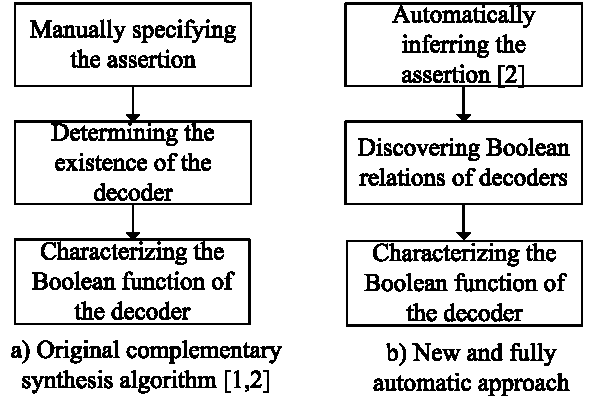
\includegraphics[width=0.35\textwidth]{flow}
% \end{center}
% \caption{The original and new flows of complementary synthesis}
%   \label{flow}
% \end{figure}

For example,
for the two decoders of XFI discovered by our algorithm,
their corresponding precondition formulas refer to only three pins,
only two of which have different values.
Therefore,
to select the correct decoder,
one only needs to find out the meaning of these two pin,
instead of all 120 pins.
More details can be found in the experimental results section,
which indicates that our algorithm can significantly save the human effort in specifying assertion and selecting decoder.
All the Experimental Results and programs can be downloaded from \url{http://www.ssypub.org}.

%We have run this algorithm on several complex encoders from industrial projects
%(e.g.,
%PCI-E\cite{PCIESPEC} and Ethernet\cite{IEEE80232002}).
%For most benchmarks,
%there exists only one decoder.
%For other benchmarks with multiple decoders,
%the user can easily select the correct one,
%by inspecting the precondition formulas
%and finding out the meaning of no more than one pin,
%instead of up to 120 pins like the original approach\cite{ShengYuShen:iccad09}.


% Only two out of our five benchmarks have no more than two decoders,
% the other three only have one decoder.
% All programs and results can be downloaded from \url{http://www.ssypub.org/exp/compsyn_fmcad11.tgz}.


\emph{The remainder of this paper is organized as follows}.
%Section \ref{sec_casestudy} explains our ideas with a simple example.
Section \ref{sec_prem} introduces background materials.
Section \ref{sec_algo} presents the algorithm that infers assertions.
% and the proof of its correctness.
% while Section \ref{sec_infer} explains how to enlarge the discovered invalid configuration value to a larger formula.
% Section \ref{sec_rmred} reduces the parameters' values discovered by Section \ref{sec_algo}.
Section \ref{sec_fdtest} discusses how to discover all decoders and characterize their precondition formulas.
Sections \ref{sec_exp} and \ref{sec_relwork} present the experimental results and related works.
Finally,
Section \ref{sec_conclude} provides the conclusion.

%\section{Case Study}\label{sec_casestudy}
%In this section,
%we will explain our ideas with a simple encoder in Fig. \ref{multidec}.
%This encoder has two constant configuration pins :
%$c_1$ and $c_2$.
%The functionality of this encoder is:
%\begin{enumerate}
% \item When $c_2\equiv 0$,
%$20$ will be assigned to $o$.
% \item Otherwise,
%if $c_1\equiv 0$,
%$i+1$ will be assigned to $o$.
% \item Otherwise,
%$i+2$ will be assigned to $o$.
%\end{enumerate}
%
%The \emph{first} step of our algorithm finds out that,
%when $c_2\equiv 0 \wedge c_1\equiv 0$,
%it can not determine the value of $i$ from $o$,
%because the latter one is always $20$.
%\textbf{Therefore},
%it tries to enlarge this formula with Craig interpolation,
%and finds out that the resulted formula $c_2\equiv 0$ covers more configuration values that can lead to the nonexistence of the decoder.
%By inverting this formula,
%we obtain the final assertion $c_2\equiv 1$ that can ensure the existence of the decoder.
%
%However,
%under this inferred assertion,
%there actually exists two decoders.
%One is $i\stackrel{def}{=}o-1$,
%the other is $i\stackrel{def}{=}o-2$.
%To discover these two decoders,
%the \emph{second} step of our algorithm constructs a SAT instance to test whether $\mathbb{R}$,
%the Boolean relation between $i$ and $o$,
%can be expressed as a combination of $\mathbb{D}$,
%the set of already discovered decoders.
%The encoding of this SAT instance follows the functional dependency approach proposed by Lee et al. \cite{funcdep}.
%
%$\mathbb{D}$ is empty at this time,
%\textbf{therefore} $\mathbb{R}$ can not be expressed as a combination of $\mathbb{D}$,
%and this SAT instance will be satisfiable.
%Lets assume that its satisfying assignment is  $c_2\equiv 1 \wedge c_1\equiv 0$.
%By asserting this assignment into $\mathbb{R}$,
%we get the Boolean relation of the decoder $i\stackrel{def}{=}o-1$,
%and insert it into $\mathbb{D}$.
%
%Now the \emph{second} step of our algorithm constructs the second SAT instance to test whether $\mathbb{R}$ can be expressed as a combination of the already discovered decoder,
%that is,
%$i\stackrel{def}{=}o-1$.
%This new SAT instance will be satisfiable again,
%and the new satisfying assignment is $c_2\equiv 1 \wedge c_1\equiv 1$.
%By asserting this assignment into $\mathbb{R}$,
%we get the Boolean relation of the other decoder $i\stackrel{def}{=}o-2$,
%
%Again,
%the \emph{second} step of our algorithm constructs a third SAT instance to test whether $\mathbb{R}$ can be expressed as a combination of the two discovered decoders.
%At this time,
%this SAT instance will be unsatisfiable,
%which means no more decoder can be found.
%
%With the functional dependency approach proposed by Lee et al. \cite{funcdep},
%we can characterize each decoder's precondition formula,
%which represents the set of encoder's configuration values that correspond to this decoder.
%The precondition formula of the decoder $i\stackrel{def}{=}o-1$ is $c_1\equiv 0$,
%and the precondition formula of the decoder $i\stackrel{def}{=}o-2$ is $c_1\equiv 1$.
%
%At this point,
%by inspecting these two precondition formulas,
%we know that their essential difference is the assignment to $c_1$.
%\textbf{Therefore},
%we only need to find out the meaning of $c_1$ by reading the documentation or source code,
%instead of both $c_1$ and $c_2$ like the original approach \cite{ShengYuShen:iccad09}.
%
%Some larger benchmark,
%such as XFI in Subsection \ref{subsec_expbench},
%has more than 100 configuration pins.
%Our approach can significantly save the user's efforts by reducing the number of pins whose meaning need to be manually find out.
%
%\begin{figure}[t]
%\begin{center}
%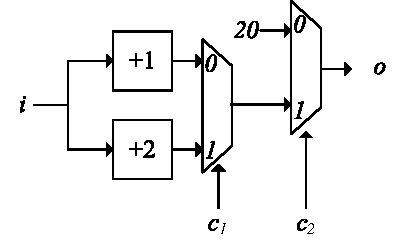
\includegraphics[width=0.35\textwidth]{multidec}
%\end{center}
%\caption{The encoder used to explain our ideas}
%  \label{multidec}
%\end{figure}

\section{Preliminaries}\label{sec_prem}

%\subsection{Propositional satisfiability and related topics}\label{subsec_SAT}
To save space,
we assume the readers' familiarity with propositional satisfiability (SAT),
cofactoring \cite{Cofact},
Craig interpolant generation \cite{interp_McMillan},
and functional dependency \cite{funcdep}.

%
%
%The Boolean value set is denoted as $\mathbb{B}=\{0,1\}$.
%For a Boolean formula $F$ over a variable set $V$,
%the propositional satisfiability problem(SAT) is to find a satisfying assignment $A:V\to \mathbb{B}$,
%such that $F$ can be evaluated to 1.
%If $A$ exists, then $F$ is satisfiable;
%otherwise,
%it is unsatisfiable.
%A SAT solver is a program that decides the existence of $A$,
%such as Zchaff\cite{CHAFF},
%Grasp\cite{grasp},
%Berkmin\cite{BERKMIN},
%and MiniSAT\cite{EXTSAT}.
%Normally,
%the formula $F$ is represented in the conjunctive normal form(CNF),
%where a formula is a conjunction of its clause set,
%and a clause is a disjunction of its literal set,
%and a literal is a variable or its negation.
%A CNF formula is also called a SAT instance.
%
%
%%\subsection{Cofactoring}\label{subsec_pre_cofact}
%
%For a Boolean function $f:\mathbb{B}^n\to \mathbb{B}$,
%we use $supp(f)$ to denote its support set $\{v_1\dots v_n\}$.
%According to Ganai et al. \cite{Cofact},
%the positive and negative cofactors of $f(v_1\dots v\dots v_n)$ with respect to variable
%$v$ are $f_v=f(v_1\dots 1\dots v_n)$ and $f_{\overline{v}}=f(v_1\dots 0\dots v_n)$
%respectively.
%% Existential quantification of $f(v_1\dots v\dots v_n)$ with respect to a
%% variable $v$ is $\exists v f=f_v+f_v’$.
%\emph{Cofactoring} is the action that applies 1 or 0 to $v$ to get $f_v$ or $f_{\overline{v}}$.
%
%
%%\subsection{Craig Interpolation}\label{subsec_pre_interp}
%Craig\cite{Craig} had proved the following theorem:
%
%\begin{theorem}[Craig Interpolation Theorem]\label{thm_craig}
%Given two Boolean formulas $\phi_A$ and $\phi_B$,
%with $\phi_A\wedge \phi_B$ unsatisfiable,
%there exists a Boolean formula $\phi_I$ referring only
%to the common variables of $\phi_A$ and $\phi_B$ such that $\phi_A\to \phi_I$
%and $\phi_I\wedge \phi_B$ is unsatisfiable.
%$\phi_I$ is referred to as the \emph{interpolant} of $\phi_A$ with respect to $\phi_B$.
%\end{theorem}
%
%In the remainder of this paper,
%we will use the algorithm proposed by McMillan\cite{interp_McMillan} to generate interpolant from the proof of unsatisfiability,
%which is generated by MiniSAT\cite{EXTSAT}.
%
%Given a Boolean function $f:\mathbb{B}^l\to \mathbb{B}$ and a vector of
%Boolean functions $G=(g_1, ..., g_n)$ with $g_i: \mathbb{B}^l\to \mathbb{B}$ for $i =1,\dots ,n$,
%\emph{functional dependency} \cite{funcdep} is the problem that
%finds a third Boolean function $h:\mathbb{B}^n\to \mathbb{B}$,
%such that $f(X) = h(g_1(X),\dots , g_n(X))$.
%Lee et al. \cite{funcdep} constructed a SAT instance to test whether $h$ existed,
%and used Craig interpolation \cite{interp_McMillan} to characterize it.

%we will focus on the Boolean propositional logic only,
%% There are many approaches to generate interpolants for propositional logic,
%% so please refer to Krajicek\cite{interp_Krajicek},
%% Pudlak\cite{interp_Pudlak} and McMillan\cite{interp_McMillan} for more details.

%\subsection{Functional Dependency}\label{subsec_prefd}
% \textbf{Functional dependency}\cite{funcdep} is defined as:
%
% \begin{definition11}\label{def_fd}
% Given a Boolean function $f:B^m\to B$ and a vector of
% Boolean functions $G=(g_1(X), ..., g_n(X))$ with $g_i: B^m\to B$ for $i =1,\dots ,n$,
% over the same set of variable vector $X = (x_1,\dots , x_m)$, we
% say that $f$ \textbf{functionally depends} on $G$ if there exists a Boolean
% function $h: B_n\to B$, called the dependency function, such that
% $f(X) = h(g_1(X),\dots , g_n(X))$.
% %We call functions $f$, $G$, and $h$ the \textbf{target
% %function}, \textbf{base functions}, and \textbf{dependency function}, respectively.
% \end{definition11}

% Lee et al. \cite{funcdep} proposes to test functional dependency by constructing a SAT instance and proving its unsatisfiability.

% \subsection{Recurrence Diameter}
%
% A circuit can be modeled by a Mealy machine \cite{MEALY}.
%
% \begin{definition11}\label{MealyFSM_old}%\addtolength{\itemsep}{-0.5\baselineskip}
% %{\setlength{\baselineskip}{0.5\baselineskip}
% \textbf{Mealy finite state machine} is a 5-tuple $M=(S,s_0,I,O,T)$,
% consisting of a finite state set $S$,
% an initial state $s_0\in S$,
% a finite set of input letters $I$,
% a finite set of output letters $O$,
% a transition function $T: S\times I\to S\times O$ that computes the next state and output letter from the current state and input letter.
% %}
% \end{definition11}
%



% Obviously,
% a state sequence longer than $uirrd(M)$ must be a loop-like path.


%\subsection{Determining the decoder's existence}\label{subsec_chkextdec}
% Complementary synthesis\cite{ShengYuShen:iccad09} includes two steps:
% determining the existence of the decoder and characterizing its Boolean function.
% We will only introduce the first step here.
The encoder is modeled using \emph{Mealy finite state machine with configuration} $M=(S,s_0,I,C,O,T)$,
consisting of a finite state set $S$,
an initial state $s_0\in S$,
a finite input letter set $I$,
a finite configuration letter set $C$,
a finite output letter set $O$,
and a transition function $T: S\times I\times C\to S\times O$ that computes the next state
and output letter from the current state,
input letter,
and configuration letter.
%}

%\begin{figure}[t]
%\centering
%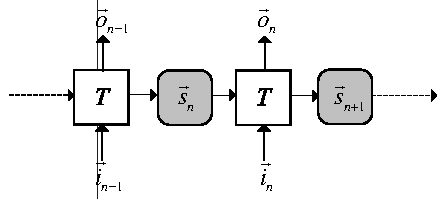
\includegraphics{mealy}
%\caption{Mealy finite state machine with configuration}
%\label{mealy}
%\end{figure}

%As shown in Fig. \ref{mealy},
%% as well as in the remainder of this paper,
%the state is represented as a gray round corner box,
%and the transition function $T$ is represented as a white rectangle.
We denote the state, input letter, output letter, and configuration letter at the $n$-th cycle as $s_n$, $i_n$, $o_n$, and $c_n$,respectively.
We further denote the sequence of state, input letter, output letter, and configuration letter from the $n$-th to the $m$-th cycle as $s_n^m$, $i_n^m$, $o_n^m$, and $c_n^m$, respectively.
%A \emph{path} is a state sequence $s_n^{m}$ with $\exists i_jo_jc:(s_{j+1},o_j)\equiv T(s_j,i_j,c)$ for all $n\le j< m$.
%A \emph{loop} is a path $s_n^{m}$ with $s_n\equiv s_m$.
% A \textbf{loop-like path} is a state sequence $s_n^{m}$ with $s_i\equiv s_j$,
% where $n\le i< j\le m$.

%The state variables recurrence diameter\cite{RecDiam} of the Mealy machine $M$,
%% denoted by $rrd(M)$,
%is the longest path without loop in $M$ starting from an initial state.
% \begin{equation}\label{equ_svrd}
% rrd(M)\stackrel{def}{=}\max\{i|\exists s_0 \dots s_i:
% I(s_0)\wedge \bigwedge^{i-1}_{j=0}T(s_j,s_{j+1})\wedge\bigwedge^{i-1}_{j=0}\bigwedge^{i}_{k=j+1}s_{j}\ne s_{k}\}
% \end{equation}
%The \emph{uninitialized recurrence diameter} of a Mealy machine $M$ is defined
%as the longest path without loop.
%}

%\begin{equation}\label{equ_uisvrd}
%\begin{split}
%uirrd(M)\stackrel{def}{=}\max\{i|\exists s_0 \dots s_i  i_0 \dots i_i o_0 \dots o_ic:\\
%\bigwedge^{i-1}_{j=0}(s_{j+1},o_j)\equiv T(s_j,i_j,c)\wedge\bigwedge^{i-1}_{j=0}\bigwedge^{i}_{k=j+1}s_{j}\ne s_{k}\}
%\end{split}
%\end{equation}

%The only difference between this definition and Kroening's state variables recurrence diameter\cite{RecDiam} is that
%our $uirrd$ does not consider the initial state.
%We only used this definition to prove our theorems.
%Our algorithm does not compute it.

% \begin{definition11}\label{def_ass}
\emph{An assertion (or formula) on configuration pins} is defined as a configuration letter set $R$.
%For a configuration letter $c$,
$R(c)$ means $c\in R$.
If $R(c)$ holds,
we also say that $R$ covers $c$.
% \end{definition11}

% As shown in Fig. \ref{fig_pcln}a),
% the decoder exists if there are three parameters $p$, $d$ and $l$,
% such that $i_n$ of the encoder can be uniquely determined by the output sequence $o_{n+d-l}^{n+d-1}$.
% $d$ is the relative delay between $o_{n+d-l}^{n+d-1}$ and $i_n$,
% while $l$ is the length of $o_{n+d-l}^{n+d-1}$,
% and $p$ is the length of the prefix path used to rule out some unreachable states.
% This can be formally defined as:

The decoder exists if the encoder's input can be uniquely determined by its output.
As shown in Fig. \ref{fig_pcln}a),
this can be formally defined as follows.

\begin{definition11}\label{def_pcc}%\addtolength{\itemsep}{-0.5\baselineskip}
%{\setlength{\baselineskip}{0.5\baselineskip}
\emph{Parameterized complementary condition (PC)}:
For encoder $E$,
assertion $R$,
and parameters $p$, $d$, and $l$,
$E\vDash PC(p,d,l,R)$ holds if
$i_n$ can be uniquely determined by $o_{n+d-l}^{n+d-1}$,
and $R$ covers the constant configuration letter $c$.
This amounts to the unsatisfiability of $F_{PC}(p,d,l,R)$ in Equation (\ref{uniqt1}).
%We further define $E\vDash PC(R)$ as $\exists p,d,l:E\vDash PC(p,d,l,R)$.
\end{definition11}


\begin{equation}\label{uniqt1}
\begin{split}
&F_{PC}(p,d,l,R)\stackrel{def}{=}\\
&\left\{
\begin{array}{cc}
&\bigwedge_{m=n-p}^{n+d-1}
\{
(s_{m+1},o_m)\equiv T(s_m,i_m,c)
\}
\\
\wedge&\bigwedge_{m=n-p}^{n+d-1}
\{
(s'_{m+1},o'_m)\equiv T(s'_m,i'_m,c)
\}
\\
\wedge&\bigwedge_{m=n+d-l}^{n+d-1}o_m\equiv o'_m \\
\wedge& i_n\ne i'_n \\
% \wedge&\bigwedge_{x=n-p}^{n+d-1}c_x\equiv c \\
% \wedge&\bigwedge_{x=n-p}^{n+d-1}c_x'\equiv c \\
\wedge& R(c)
\end{array}
\right\}
\end{split}
\end{equation}

%This definition is the same as that of Subsection \ref{subsec_chkextdec} and paper \cite{ShengYuShen:iccad09}.

% The 2nd to 5th lines of Equation (\ref{uniqt1}) correspond to Condition 1 of Definition \ref{def_pcc}.
Lines 2 and 3 of Equation (\ref{uniqt1}) correspond to two state sequences of $E$, respectively.
% The only difference between them is that a prime is appended to every variable in Line 3 .
Line 4 forces the output sequences of these two state sequences to be the same,
while Line 5 forces their input letters to be different.
% At the same time,
% the last three lines of Equation (\ref{uniqt1}) correspond to Condition 2 of Definition \ref{def_pcc}.
% The 6th and the 7th lines constrain that all configuration letters are equal to $c$,
The last line constrains $c$ to be covered by $R$.
% 
% \begin{figure}[t]
% \begin{center}
% 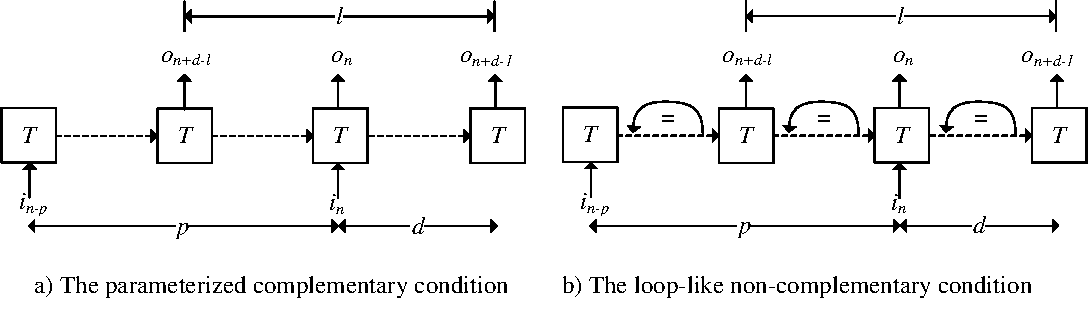
\includegraphics[width=0.5\textwidth]{pcln}
% \end{center}
% \caption{The parameterized complementary condition and the loop-like non-complementary condition}
%   \label{fig_pcln}
% \end{figure}


The algorithm based on checking $PC$\cite{ShengYuShen:iccad09} just enumerates all combinations of $p$, $d$, and $l$,
from small to large,
until $F_{PC}(p,d,l,R)$ becomes unsatisfiable,
which means that the decoder exists.


\section{A Halting Algorithm to Infer Assertion}\label{sec_algo}
In Subsection \ref{subsec_chknonext},
we first define how to determine the decoder's nonexistence for a particular configuration letter.
% This will be discussed in Subsection \ref{subsec_chknonext}.
% while the proof of its correctness is presented in Subsection \ref{subsec_correctness}.
% Based on this result,
And then,
in Subsection \ref{subsec_algo},
we introduce the algorithm that infers assertion
by iteratively detecting and removing all invalid configuration letters.

\subsection{Determining the decoder's nonexistence}\label{subsec_chknonext}


According to Definition \ref{def_pcc},
the decoder exists for a set of configuration letters $R$ if there is a parameter value tuple $<p,d,l>$ that makes
$E\vDash PC(p,d,l,R)$ holds true.
% such that every path longer than $p$ always reaches a particular state $s_n$,
% in which the input letter $i_n$ can be uniquely determined by the output sequence $o_{n+d-l}^{n+d-1}$.
Therefore,
intuitively,
the decoder does not exist if for every parameter value tuple $<p,d,l>$,
we can always find another tuple $<p',d',l'>$ with $p'>p$,$l'>l$ and $d'>d$,
such that $E\vDash PC(p',d',l',R)$ does not hold.

This case can be detected by the SAT instance shown in Figure \ref{fig_pcln}b),
which is similar to that of Figure \ref{fig_pcln}a),
except that three new constraints are inserted to detect loops on $s_{n-p}^{n+d-l}$,$s_{n+d-l+1}^n$, and $s_{n+1}^{n+d}$.

%\begin{figure}[t]
%\begin{center}
%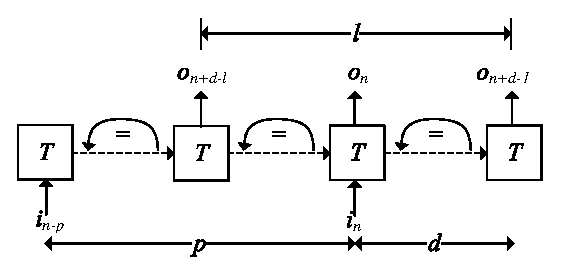
\includegraphics[width=0.45\textwidth]{doubleloop}
%\end{center}
%\caption{The loop-like non-complementary condition}
%  \label{fig_double_loop}
%\end{figure}

% If this SAT instance is satisfiable,
% for any parameter value $<p,d,l>$,
% we can unfold these three loops until we find $<p',d',l'>$ that is larger than $<p,d,l>$.
% This unfolded instance is still satisfiable,
% which means $E\vDash PC(p',d',l',R)$ does not hold.
% \textbf{Therefore},
% the decoder does not exist.
Thus,
the decoder's nonexistence can be determined by:

%According to Line 2 and 3 of Equation (\ref{uniqt1}),
%there are actually two paths,
%\textbf{therefore} we need to detect these loops on both of them,
%i.e.,
%on the product machine $M^2$ defined below:
%
%\begin{definition11}%\addtolength{\itemsep}{-0.5\baselineskip}
%%{\setlength{\baselineskip}{0.5\baselineskip}
%\emph{Product machine:} For Mealy machine $M=(S,s_0,I,C,O,T)$,
%its product machine is $M^2=(S^2,s_0^2,I^2,C^2$ $,O^2,T^2)$,
%where
%$T^2$ is defined as $(<s_{m+1},s'_{m+1}>,<o_m,o'_m>)=T^2(<s_m,s'_m>,<i_m,i'_m>,<c_m,c'_m>)$ with $(s_{m+1},o_m)=T(s_m,i_m,c_m)$ and $(s'_{m+1},o'_m)=T(s'_m,i'_m,c'_m)$.
%\end{definition11}


\begin{definition11}\label{def_lnc}%\addtolength{\itemsep}{-0.5\baselineskip}
%{\setlength{\baselineskip}{0.5\baselineskip}
\emph{Loop-like Non-complementary Condition (LN):} For encoder $E$,
%assume its product machine is $M^2=(S^2,s_0^2$ $,I^2,C^2,O^2,T^2)$,
$E\vDash LN(p,d,l,R)$ holds if
$i_n$ can not be uniquely determined by $o_{n+d-l}^{n+d-1}$ on $s_{n-p}^{n+d-1}$,
and there are loops on $s_{n-p}^{n+d-l}$, $s_{n+d-l+1}^n$, and $s_{n+1}^{n+d}$.
This amounts to the satisfiability of $F_{LN}(p,d,l,R)$ in Equation (\ref{uniqln}).
%We further define $E\vDash LN(R)$ as $\exists p,d,l:E\vDash LN(p,d,l,R)$.
\end{definition11}


\begin{equation}\label{uniqln}
\begin{split}
&F_{LN}(p,d,l,R)\stackrel{def}{=}\\
&\left\{
\begin{array}{cc}
&F_{PC}(p,d,l,R) \\
\wedge& \bigvee_{x=n-p}^{n+d-l-1}\bigvee_{y=x+1}^{n+d-l} \{s_x\equiv s_y\wedge s'_x\equiv s'_y\} \\
\wedge& \bigvee_{x=n+d-l+1}^{n-1}\bigvee_{y=x+1}^{n} \{s_x\equiv s_y\wedge s'_x\equiv s'_y\} \\
\wedge& \bigvee_{x=n+1}^{n+d-1}\bigvee_{y=x+1}^{n+d} \{s_x\equiv s_y\wedge s'_x\equiv s'_y\}
\end{array}
\right\}
\end{split}
\end{equation}

%By comparing Equation (\ref{uniqt1}) and (\ref{uniqln}),
%it is obvious that their only difference lies in the last three newly inserted lines in (\ref{uniqln}),
%which will be used to detect loops on the following three paths shown in Figure \ref{fig_pcln}b):
%\begin{equation}
%\begin{array}{c}
%Prefix_{p,d,l}=(s^2)_{n-p}^{n+d-l} \\
%Left_{p,d,l}=(s^2)_{n+d-l+1}^n \\
%Right_{p,d,l}=(s^2)_{n+1}^{n+d}
%\end{array}
%\end{equation}

% Thus,
% we have the following theorem:
%
% \begin{theorem}\label{thm_pcln_exclusive}
% $E\vDash LN(R)\leftrightarrow \neg \{E\vDash PC(R)\}$
% \end{theorem}
%
% The proof of its correctness can be found in \cite{ShengYuShen:iccad11}.

\subsection{Algorithm implementation}\label{subsec_algo}
% Theorems \ref{thm_pc_nln} and \ref{thm_nln_pc} show that,
% we can enumerate all combinations of $<p,d,l>$ from small to large,
% and check $E\vDash PC(p,d,l,R)$ and $E\vDash LN(p,d,l,R)$ in every iteration.
% This process will eventually terminate with one and only one answer between $E\vDash PC(R)$ and $E\vDash LN(R)$.
% The implementation of this algorithm will be presented below.

\begin{algorithm}
\caption{InferAssertion}
\label{algo_pcln}
\begin{algorithmic}[1]
\STATE $NA=\{\}$
\FOR{$x=0\to \infty$}
\STATE $<p,d,l>=<2x,x,2x>$
\label{algo_pcln_pdl}
\IF{$F_{PC}(p,d,l,\bigwedge_{na\in NA}\neg na)$ is unsatisfiable}
\label{algo_pcln_pc}
\STATE Halt. The final assertion is $\bigwedge_{na\in NA}\neg na$, the decoder exists if it is satisfiable.
%\IF{$\bigwedge_{na\in NA}\neg na$ is satisfiable}
%\STATE decoder exists with final assertion $\bigwedge_{na\in NA}\neg na$
%\ELSE
%\STATE decoder does not exist
%\ENDIF
\ELSE
\WHILE{$F_{LN}(p,d,l,\bigwedge_{na\in NA}\neg na)$ is satisfiable}
\label{algo_pcln_lnc}
\STATE Assume $A(c)$ is $c$'s satisfying assignment leading to the decoder's nonexistence.
\label{algo_pcln_Ac}
\STATE $na\leftarrow InferCoveringFormula(A(c))$
\label{algo_pcln_nainfer}
\STATE $NA\leftarrow NA\cup \{na\}$
\label{algo_pcln_ruleout}
\ENDWHILE
\ENDIF
\ENDFOR
\end{algorithmic}
\end{algorithm}

% In Line 1 of Algorithm \ref{algo_pcln},
% $NA$ will be used to record all inferred formulas that can lead to the nonexistence of the decoder.
% They are all inferred by the procedure $InferCovering$ $Formula$ in Line 14,
% whose functionality is to infer a formula that can cover not only $c$,
% but also many other configuration letters leading to the nonexistence of the decoder.
% More details of this procedure will be presented in Section \ref{sec_infer}.
%
% Line 3 ensures that the length of $Prefix_{p,d,l}$,$Left_{p,d,l}$ and $Right_{p,d,l}$ are all set to $x$,
% whose value is enumerated in Line 2.
% In this way,
% many redundant combinations of $p$,$d$ and $l$ are no longer need to be tested.
% Thus, the performance of this algorithm can be significantly boosted.
%
% Line 4 means the input letter can be uniquely determined by the output sequence with the assertion $\bigwedge_{na\in NA}\neg na$.
% Line 5 means that there is at least one configuration letter that can lead to the existence of the decoder,
% and the final assertion is $\bigwedge_{na\in NA}\neg na$ in the 6th line.
%
% Line 7 means that the inferred assertion $\bigwedge_{na\in NA}\neg na$ has ruled out all configuration letters,
% that is,
% no configuration letter can lead to the existence of the decoder.
% There must be some bugs in the encoder.
%
% Line 11 means that the decoder does not exist with the configuration letter $c$ in Line 12.
% We need to rule out $c$ such that Algorithm \ref{algo_pcln} can continue searching for other configuration letters that may lead to the existence of the decoder.
% The procedure $InferCoveringFormula$ in Line 14 will be used to infer a formula $na$ that covers not only $c$,
% but also a large set of invalid configuration letters.
% They will be ruled out in Line 15.

Algorithm \ref{algo_pcln} is used to infer assertion on configuration pins that can lead to the decoder's existence.
Intuitively,
it iteratively tests all combinations of $<p,d,l>$ in Line \ref{algo_pcln_pdl}.
For every $A(c)$ found in Line \ref{algo_pcln_Ac} that can lead to the decoder's nonexistence,
a larger set of such configuration letters are discovered by the procedure $InferCoveringFormula$ in Line \ref{algo_pcln_nainfer},
and ruled out in Line \ref{algo_pcln_ruleout}.
This loop is repeated until the formula $F_{PC}$ in Line \ref{algo_pcln_pc} is unsatisfiable.
%At this point,
%if this assertion is satisfiable,
%then the decoder exists.
%Otherwise,
%the decoder does not exist.

$InferCoveringFormula$ uses cofactoring \cite{Cofact} to assert the satisfying assignments of $i_{n-p}^{n+d-1}$,
$(i')_{n-p}^{n+d-1}$, $s_{n-p}$, and $(s')_{n-p}$ back to $F_{LN}$,
and then uses Craig interpolation \cite{interp_McMillan} to characterize a larger set of invalid configuration letters.
More details can be found in \cite{ShengYuShen:iccad11},
which had proved that Algorithm \ref{algo_pcln} is a halting one.
%We can prove that Algorithm \ref{algo_pcln} is a halting one.
%\begin{theorem}\label{thm_pcln_halt}
%Algorithm \ref{algo_pcln} is a halting algorithm.
%\end{theorem}
%\begin{proof}
%According to Theorems \ref{thm_pcln_exclusive},
%Algorithm \ref{algo_pcln} will eventually reach Line \ref{algo_pcln_pc} or \ref{algo_pcln_lnc}.
%
%In the former case,
%this algorithm will halt at Line \ref{algo_pcln_halt}.
%
%In the latter case,
%a new formula $na$ will be inferred,
%which will cover the configuration letter $A(c)$.
%Because the number of such $A(c)$ is finite,
%all of them will eventually be ruled out by $\bigwedge_{na\in NA}\neg na$.
%Then Algorithm \ref{algo_pcln} will eventually reach Line \ref{algo_pcln_pc},
%and halt at Line \ref{algo_pcln_halt}.
%\end{proof}

%\subsection{The Implementation of $InferCoveringFormula$}\label{subsec_infer}
%$InferCoveringFormula$ includes three steps:
%
%\subsubsection{}
%First,
%we need to move the 4th line and the last three lines of Equation (\ref{uniqln}) into a new subformula:
%
%\begin{equation}\label{uniqln_subg}
%\begin{split}
%&G(p,d,l)\stackrel{def}{=}\\
%&\left\{
%\begin{array}{cc}
%&\bigwedge_{m=n+d-l}^{n+d-1}o_m\equiv o'_m \\
%\wedge& \bigvee_{x=n-p}^{n+d-l-1}\bigvee_{y=x+1}^{n+d-l} \{s_x\equiv s_y\wedge s'_x\equiv s'_y\} \\
%\wedge& \bigvee_{x=n+d-l+1}^{n-1}\bigvee_{y=x+1}^{n} \{s_x\equiv s_y\wedge s'_x\equiv s'_y\} \\
%\wedge& \bigvee_{x=n+1}^{n+d-1}\bigvee_{y=x+1}^{n+d} \{s_x\equiv s_y\wedge s'_x\equiv s'_y\}
%\end{array}
%\right\}
%\end{split}
%\end{equation}
%
%And then,
%$F_{LN}$ can be transformed into :
%\begin{equation}\label{uniqln_new}
%\begin{split}
%&F'_{LN}(p,d,l,R)\stackrel{def}{=}\\
%&\left\{
%\begin{array}{cc}
%&\bigwedge_{m=n-p}^{n+d-1}
%\{
%(s_{m+1},o_m)\equiv T(s_m,i_m,c_m)
%\}
%\\
%\wedge&\bigwedge_{m=n-p}^{n+d-1}
%\{
%(s'_{m+1},o'_m)\equiv T(s'_m,i'_m,c'_m)
%\}
%\\
%\wedge& i_n\ne i'_n \\
%\wedge&\bigwedge_{x=n-p}^{n+d-1}c_x\equiv c \\
%\wedge&\bigwedge_{x=n-p}^{n+d-1}c_x'\equiv c \\
%\wedge& R(c) \\
%\wedge& t\equiv G(p,d,l)
%\end{array}
%\right\}
%\end{split}
%\end{equation}
%
%%It is obvious that $F_{LN}$ and $F'_{LN}\wedge t\equiv 1$ is equisatisfiable.
%
%%According to Figure \ref{fig_pcln}b),
%$F'_{LN}$ defines a function $f':S^{2}\times I^{(d+p)*2}\times C\to \mathbb{B}$,
%whose support set is $\{s_{n-p},s'_{n-p},i_{n-p}^{n+d-1},(i')_{n-p}^{n+d-1},c\}$,
%and its output is the variable $t$ in the last line of Equation (\ref{uniqln_new}).
%
%\subsubsection{}
%%According to Line \ref{algo_pcln_lnc} of Algorithm \ref{algo_pcln},
%%$F_{LN}$ is satisfiable.
%We assume that $A$ is the satisfying assignment of $F_{LN}$,
%and assert the value of $i_{n-p}^{n+d-1}$, $(i')_{n-p}^{n+d-1}$, $s_{n-p}$ and $(s')_{n-p}$ into formula $F'_{LN}$,
%and get :
%
%\begin{equation}\label{equ_char}
%F"_{LN}(c,t)\stackrel{def}{=}
%\left\{
%\begin{array}{cc}
%& F'_{LN}\\
%\wedge& i_{n-p}^{n+d-1}\equiv A(i_{n-p}^{n+d-1})\\
%\wedge& (i')_{n-p}^{n+d-1}\equiv A((i')_{n-p}^{n+d-1})\\
%\wedge& s_{n-p}\equiv A(s_{n-p})\\
%\wedge& (s')_{n-p}\equiv A((s')_{n-p})
%\end{array}
%\right\}
%\end{equation}
%
%Now,
%$F"_{LN}$ defines another function $f"$,
%whose support set is reduced to $c$.
%$F"_{LN}(c,t)\wedge t\equiv 1$ is the formula that covers a set of invalid configuration letters.
%But it is still a large complicated CNF clause set.
%To reduce its size,
%we need the characterizing algorithm in the next subsection.
%
%\subsubsection{}
%
%We then encode $F"_{LN}(c,t)$ into the CNF format,
%and denote it as $CNF(F"_{LN}(c,t))$.
%Assume $CNF'(F"_{LN}(c,t'))$ is a copy of $CNF(F"_{LN}(c,t))$.
%%They share the same variable index for $c$,
%%while all other variables are encoded independently.
%Thus,
%we can construct formula $\phi_A$ and $\phi_B$ as:
%
%\begin{equation}\label{equ_interpA}
%\begin{split}
%\phi_A\stackrel{def}{=}& CNF(F"_{LN}(c,t))\wedge t\equiv 1\\
%\phi_B\stackrel{def}{=}& CNF'(F"_{LN}(c,t'))\wedge t'\equiv 0
%\end{split}
%\end{equation}
%
%% \begin{equation}\label{equ_interpB}
%% \phi_B\stackrel{def}{=}CNF'(F"_{LN}(c,t'))\wedge t'\equiv 0
%% \end{equation}
%
%The interpolant generated from the unsatisfiable formula $\phi_A\wedge \phi_B$ characterizes a larger set of invalid configuration values.

% \section{Removing Redundancy}\label{sec_rmred}
%
% The $p$, $d$ and $l$ found by Algorithm \ref{algo_pcln} contain some redundancy,
% which can cause unnecessarily large overheads on the circuit area and on the runtime of characterizing Boolean function of the decoder.
% So,
% Algorithm \ref{algo_remove} is used to minimize $p$, $d$ and $l$ before passing it to the next algorithm.
%
% \begin{algorithm}
% \caption{$RemoveRedundancy(p,d,l,R)$}
% \label{algo_remove}
% \begin{algorithmic}[1]
% \FOR{$p'=p \to 0$}
%   \IF{$F_{PC}(p'-1,d,l,R)$ is satisfiable}
%     \STATE break
%   \ENDIF
% \ENDFOR
% \FOR{$d'=d \to 0$}
%   \IF{$F_{PC}(p',d'-1,l,R)$ is satisfiable}
%     \STATE break
%   \ENDIF
% \ENDFOR
% \FOR{$l'=1 \to l-(d-d')$}
%   \IF{$F_{PC}(p',d',l',R)$ is unsatisfiable}
%     \STATE break
%   \ENDIF
% \ENDFOR
% \PRINT \texttt{"final result is $<p',d',l'>$"}
% \end{algorithmic}
% \end{algorithm}
%
%
% This algorithm reduces the value of $p$, $d$ and $l$ iteratively,
% and tests whether the reduced values can still make $E\vDash PC(R)$ hold.
% We will not go into the details here.
%


\section{Discovering Multiple Decoders}\label{sec_fdtest}
Subsection \ref{subsec_fd_detail} introduces how to discover decoders and its correctness proof,
while Subsection \ref{subsec_charia} presents how to characterize the precondition formula of each discovered decoder,
to help the user select the correct one.

\subsection{Constructing SAT instance to discover decoders}\label{subsec_fd_detail}
% To discover the Boolean relations of all decoders,
% we need to use functional dependency test proposed by Lee et al. \cite{funcdep},
% % For a particular Boolean function $f:B^m\to B$ and a vector of
% % Boolean functions $G=(g_1(X), ..., g_n(X))$ with $g_i: B^m\to B$ for $i =1,\dots ,n$,
% whose standard definition is given in Definition \ref{def_fd}.
%
% But in this paper,
% our approach are different from that of Lee et al. \cite{funcdep} in two ways:
% \begin{enumerate}
%  \item We do not have these functions,
% only have their Boolean relations.
%  \item The functions defined by our Boolean relations have multiple output bits,
% while those functions of  Lee et al. \cite{funcdep} only have one output bit.
% \end{enumerate}

% Due to these differences,
% we need to define the functional dependency in s new way:

% We must first define the meaning of combination of Boolean relations.
%
% \begin{definition11}\label{def_combination}
% Given a Boolean relation set $\{R_{f_i}(X,Y)|0\le i\le n\}$ in which $X$ uniquely determines $Y$,
% assume the set of their corresponding function is $\{Y=f_i(X)|0\le i\le n\}$,
% we say that $R_{f_0}$ \textbf{functionally depends} on $R_{f_1},\dots,R_{f_n}$ if and only if
% $f_0$ \textbf{functionally depends} on $f_1,\dots,f_n$.
% \end{definition11}

Assume the assertion inferred by Algorithm \ref{algo_pcln} is:

\begin{equation}\label{equ_fdia}
IA\stackrel{def}{=}\bigwedge_{na\in NA}\neg na
\end{equation}

% \textbf{Therefore},
% the actual meaning of $IA$ depends on its context.
%We further assume the parameter value discovered by Algorithm \ref{algo_pcln} is $<p, d, l>$,
%and the Boolean relation that uniquely determines $i_n$ from $o_{n+d-l}^{n+d-1}$ and the configuration letter $c$ is $F_{PC}(p,d,l,IA)$.
To simplify the presentation, we denote $o_{n+d-l}^{n+d-1}$ and $i_n$ as:

\begin{equation}\label{equ_fdin}
\begin{split}
X\stackrel{def}{=}& o_{n+d-l}^{n+d-1}\\
Y\stackrel{def}{=}& i_n
\end{split}
\end{equation}
% \begin{equation}\label{equ_fdo}
% Y\stackrel{def}{=} i_n
% \end{equation}

Thus,
the Boolean relation that uniquely determines $i_n$ from $o_{n+d-l}^{n+d-1}$ and $c$ can be denoted as:

\begin{equation}\label{equ_fdR}
\mathbb{R}(c,X,Y)\stackrel{def}{=} F_{PC}(p,d,l,IA)
\end{equation}


% According to Equation (\ref{equ_fdR}),
% $R(c,o_{n+d-l}^{n+d-1},i_n)$ is the Boolean relation that uniquely determines $i_n$ from $o_{n+d-l}^{n+d-1}$.
$\mathbb{R}(c,X,Y)$ defines a mapping from $c$ and $X$ to $Y$,
which is actually a function $f$:

\begin{equation}\label{equ_fdf}
Y=f(c,X)
\end{equation}

For every configuration letter $c_i\in IA$,
there is a $\mathbb{R}_{c_i}$:

\begin{equation}\label{equ_fdRci}
\mathbb{R}_{c_i}(X,Y)\stackrel{def}{=}\mathbb{R}(c,X,Y) \wedge c\equiv c_i
\end{equation}

% Obviously,
% $R_{c_i}$ can also uniquely determined $Y$ from  $X$.
% Assume the function defined by  $R_{c_i}$ is  $f_{c_i}$:
%
% \begin{equation}\label{equ_fdfci}
% Y=f_{c_i}(X)
% \end{equation}
%
% Thus,
% $f$ can be rewritten into:
%
% \begin{equation}\label{equ_fdfrew}
% f(c,X)=\bigvee _{c_i\in IA} \{(c\equiv c_i)\wedge f_{c_i}(X)\}
% \end{equation}
%
%
% However,
% according to Table \ref{tab_res} in experimental results,
% the number of configuration pins can be as large as 120.
% This may lead to more than billions of $c_i$,
% which makes it impossible to discover $R_{c_i}$ and $f_{c_i}$ for all of them.
%
% Fortunately,
Two different $c_i$ and $c_j$ may share the same $\mathbb{R}_{c_i}$.
%that is,
%$\mathbb{R}_{c_i}\equiv \mathbb{R}_{c_j}$.
% That is,
% $IA$ can be partitioned into a small superset $SS\subseteq 2^{IA}$,
% such that:
%
% \begin{enumerate}
%  \item For every $ss_1,ss_2\in SS$,
% $ss_1\cap ss_2\equiv \phi $.
%  \item $\bigcup_{ss\in SS}\equiv IA$.
%  \item Each element $ss\in SS$ is a large set of $c_i$ that share the same $R_{c_i}$.
% \end{enumerate}
Therefore,
$IA$ can be partitioned into $\{IA_1,\dots,IA_n\}$,
such that all $c$ in the same $IA_i$ share the same $\mathbb{R}_i$,
while two $c$ and $c'$ in two different $IA_i$ and $IA_{i'}$ do not.
So we call $IA_i$ the precondition formula of $\mathbb{R}_i$,
which means $IA_i$ is the set of all configuration letters that leads to the decoder $\mathbb{R}_i$'s existence.
When there exists multiple decoders,
the user can select the correct one by inspecting $\{IA_1,\dots,IA_n\}$ characterized in Subsection \ref{subsec_charia}.


Thus,
$\mathbb{R}_i$ defines a mapping from $X$ to $Y$,
which is actually a function $f_i:X\to Y$.
Therefore,
$f$ can be rewritten as:

\begin{equation}\label{equ_fdfrewagain}
f(c,X)=\bigvee _{i=1}^{n} \{IA_i(c)\wedge f_i(X)\}
\end{equation}
Complementary Synthesis for High Speed Serial Communication Applications
%
% For function $f$,
% we denote its Boolean relation,
% its input variable set and its output variable set as $R_f$, $X$ and  $Y$,
% respectively.
% For function $g_i$,
% we denote its Boolean relation as $R_{g_i}$,
% and its output variable set as $Y_i$.
% Obviously its input variable set is still $X$.

% \begin{figure}[t]
% \centering
% 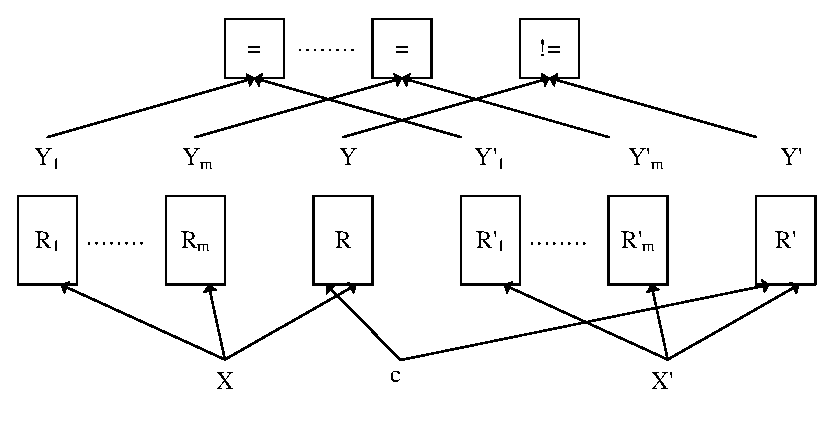
\includegraphics[width=0.45\textwidth]{fdtest}
% \caption{The SAT instance that discovers decoders}
% \label{fig_fdtest}
% \end{figure}

Thus,
our task here is to find out the set $\{\mathbb{R}_1,\dots,\mathbb{R}_n\}$ step--by--step.
Assume that we have already discovered a set of decoders' Boolean relations $\{\mathbb{R}_1,\dots,\mathbb{R}_{m}\}$.
To test whether it contains $\{\mathbb{R}_1,\dots,\mathbb{R}_n\}$,
that is,
whether all decoders have already been discovered,
we construct the following SAT instance,
which is also shown in Fig. \ref{fig_fdtest}:


% \begin{equation}\label{equ_fdtest}
% \begin{split}
% &FD(R,IA'')\stackrel{def}{=}\\
% &\left\{
% \begin{array}{cc}
%       & R(c,X,Y)\wedge \bigwedge_{i=1}^{m}R_i(X,Y_i)  \\
% \wedge& R'(c,X',Y') \wedge \bigwedge_{i=1}^{m}R'_i(X',Y'_i)  \\
% \wedge&\bigwedge_{i=1}^{m}Y_i\equiv Y'_i\\
% \wedge& Y\ne Y'
% \end{array}
% \right\}
% \end{split}
% \end{equation}

\begin{equation}\label{equ_fdtest}
\left\{
\begin{array}{cc}
      & \mathbb{R}(c,X,Y)\wedge \bigwedge_{i=1}^{m}\mathbb{R}_i(X,Y_i)  \\
\wedge& \mathbb{R}'(c,X',Y') \wedge \bigwedge_{i=1}^{m}\mathbb{R}'_i(X',Y'_i)  \\
\wedge&\bigwedge_{i=1}^{m}Y_i\equiv Y'_i\\
\wedge& Y\ne Y'
\end{array}
\right\}
\end{equation}

Line 1 of Equation (\ref{equ_fdtest}) represents the Boolean relations in $\{\mathbb{R}_1,\dots,\mathbb{R}_{m}\}$ and $\mathbb{R}$.
Line 2 is a copy of Line 1.
The only common variable shared by them is $c$.
% Line 4 forces them to share the same configuration letter $c$.
Line 3 forces all $Y_i$ and $Y'_i$ to take on the same values,
while the last line forces $Y$ and $Y'$ to be different.

% \subsection{Proof of Correctness}\label{subsec_fd_proof}
The following theorem proves that,
if Equation (\ref{equ_fdtest}) is unsatisfiable,
then all decoders have been discovered.

\begin{theorem}\label{thm_fdok}
If Equation (\ref{equ_fdtest}) is unsatisfiable,
then $\{\mathbb{R}_1,\dots,\mathbb{R}_{m}\}$ contains $\{\mathbb{R}_1,\dots,\mathbb{R}_{n}\}$.
\end{theorem}
\begin{proof}
The proof is by contradiction.
Assume $\mathbb{R}_n\notin \{\mathbb{R}_1,\dots,\mathbb{R}_m\}$,
and $IA_n$ is its corresponding set of configuration letters,
and $c_n\in IA_n$.

We can construct an assignment $A$ such that $A(c)\equiv c_n$.
Thus,
we have $\{\mathbb{R}(c,X,Y)\wedge A(c)\equiv c_n\} \equiv \mathbb{R}_n(X,Y)$,
that is,
we can change $\mathbb{R}$ and $\mathbb{R}'$ shown in Fig. \ref{fig_fdtest} to $\mathbb{R}_n$ with $A$.

As $\mathbb{R}_n\notin \{\mathbb{R}_1,\dots,\mathbb{R}_m\}$,
there must be an assignment $A'$,
such that when we assign $A'(X)$ to $X$ and $A'(X')$ to $X'$,
we can make both $\bigwedge_{i=1}^{m}Y_i\equiv Y'_i$ and $Y\ne Y'$ hold.

Therefore,
by combining $A$ and $A'$,
Equation (\ref{equ_fdtest}) becomes satisfied.
This contradiction concludes the proof.
\end{proof}



On the other hand,
if Equation (\ref{equ_fdtest}) is satisfiable,
we need to prove the following theorem.

\begin{theorem}\label{thm_fdok1}
If Equation (\ref{equ_fdtest}) is satisfiable,
then there must be at least one decoder that has not been discovered.
\end{theorem}
\begin{proof}
The proof is by contradiction.
Assume that all decoders have already been discovered,
that is,
$\{\mathbb{R}_1,\dots,\mathbb{R}_{m}\}$ contains $\{\mathbb{R}_1,\dots,\mathbb{R}_{n}\}$.
Thus,
for any assignment $A$ that makes the first three lines of Equation (\ref{equ_fdtest}) satisfied,
we have:

% This means that the function $f$ can be rewritten as:
% \begin{equation}\label{equ_fdfrewagain1}
% f(c,X)=\bigvee _{i=1}^{m} \{IA_i(c)\wedge f_i(X)\}
% \end{equation}


\begin{equation}\label{equ_fdfrewagain2}
Y=\bigvee _{i=1}^{m} \{IA_i(c)\wedge Y_i\}=\bigvee _{i=1}^{m} \{IA_i(c)\wedge Y'_i\}=Y'
\end{equation}

Thus,
the last line of Equation (\ref{equ_fdtest}) will never be satisfied.
Therefore,
Equation (\ref{equ_fdtest}) is unsatisfiable.
This contradiction concludes the proof.
\end{proof}

With the satisfying assignment $A$,
%$c_{m+1}=A(c)$ is a newly discovered configuration letter,
$\mathbb{R}_{m+1}$ defined below
is a newly discovered decoder's Boolean relation:

\begin{equation}\label{equ_newR}
\mathbb{R}_{m+1}\stackrel{def}{=}\mathbb{R}(c,X,Y)\wedge c\equiv A(c)
\end{equation}

%To prove that our approach does not carry out redundant work,
Theorem \ref{thm_new1} proves that $\mathbb{R}_{m+1}$ hasn't been discovered before:

\begin{theorem}\label{thm_new1}
$\mathbb{R}_{m+1}\notin \{\mathbb{R}_1,\dots,\mathbb{R}_m\}$
\end{theorem}
\begin{proof}
The proof is by contradiction.
Assume that there is $0\le i\le m$ such that $\mathbb{R}_i\equiv \mathbb{R}_{m+1}$.

As $\mathbb{R}_i$ can uniquely determine $Y$ from $X$,
while $\mathbb{R}$ can uniquely determine $Y$ from $X$ as well as $c$,
and  $\mathbb{R}_{m+1}\equiv \mathbb{R}_i$,
it is obvious that we can make $Y\equiv Y_i$ by forcing $c$ to be $A(c)$ in Equation (\ref{equ_newR}).
Similarly,
we have $Y'_i\equiv Y'$.

According to Line 5 of Equation (\ref{equ_fdtest}),
we have $Y\equiv Y_i\equiv Y'_i\equiv Y'$.
This is in contradiction with $Y\ne Y'$ in the last line of Equation (\ref{equ_fdtest}),
which concludes the proof.
\end{proof}


% On the other hand,
% we also need to prove that there is no redundancy in the set of all discovered decoders.
% That is,
% removing $R_{A(c)}$ from $R_{IA'}$ will fail the functional dependency test:
%
% \begin{theorem}[]\label{thm_new2}
% $R$ does not functionally depends on $R_{IA'}/R_{A(c)}$.
% \end{theorem}
% \begin{proof}
% haha
% \end{proof}

%\subsection{The implementation of algorithm}\label{subsec_fd_top}

Based on these discussions,
the following Algorithm \ref{algo_fd_top} describes how to discover the Boolean relations of all decoders.

\begin{algorithm}
\caption{$DiscoveringDecoders$}
\label{algo_fd_top}
\begin{algorithmic}[1]
% \STATE $R\leftarrow F_{PC}(p,d,l,\bigwedge_{na\in NA}\neg na)$
% \label{algo_fd_top_relation}
%\STATE $IA''=\{\}$
%\label{algo_fd_top_empty}
\WHILE{Equation (\ref{equ_fdtest}) is satisfiable}
\label{algo_fd_top_fdtest}
% \STATE Assume $A$ is the satisfying assignment
\STATE Insert $\mathbb{R}_{m+1}$ of Equation (\ref{equ_newR}) into $\{\mathbb{R}_1,\dots,\mathbb{R}_m\}$
\label{algo_fd_top_newrel}
\ENDWHILE
\STATE The set of decoders' Boolean relations is $\{\mathbb{R}_1,\dots,\mathbb{R}_m\}$
\end{algorithmic}
\end{algorithm}

% $R$ in Line \ref{algo_fd_top_relation} represents the Boolean relation that determines the encoder's input letter from its output sequence,
%$IA''$ in Line \ref{algo_fd_top_empty} represents the set of discovered configuration letters,
%while $R_{IA''}$ defined in Equation (\ref{equ_fdRIA2}) is the set of their corresponding Boolean relation of decoders.

% Line \ref{algo_fd_top_fdtest} means $\{\mathbb{R}_1,\dots,\mathbb{R}_m\}$ does not contain all decoders,
% there are some decoders not yet discovered.
% The detail of this test will be presented in Subsection \ref{subsec_fd_detail}.

% With the satisfying assignment $A$ returned from Equation (\ref{equ_fdtest}),
% $\mathbb{R}_{m+1}$ in Line \ref{algo_fd_top_newrel} is the newly discovered decoder's Boolean relation in Equation (\ref{equ_newR}).
% It will be inserted into $\{\mathbb{R}_1,\dots,\mathbb{R}_m\}$ to take part in the test in Line \ref{algo_fd_top_fdtest} again.

The loop in Algorithm \ref{algo_fd_top} monotonically increases the size of $\{\mathbb{R}_1,\dots,\mathbb{R}_m\}$.
As the number of decoders that compute $Y$ from $X$ is finite,
% this loop,
% and therefore,
Algorithm \ref{algo_fd_top} will eventually halt.

% \subsection{Characterizing Boolean functions of the decoders}
% With $\{\mathbb{R}_1,\dots,\mathbb{R}_m\}$,
% the ALLSAT algorithm \cite{ShengYuShen:tcad} is used to characterizes their Boolean functions.
%Its details are not presented here.

% For readers who are interested in the area and timing character of the generated decoders,
% please refer to Subsection V.B and V.C of Shen et al. \cite{ShengYuShen:tcad11}.

\subsection{Characterizing $\{IA_1,\dots,IA_{m}\}$}\label{subsec_charia}
Assume $\{\mathbb{R}_1,\dots,\mathbb{R}_{m}\}$ is the set of all decoders' Boolean relations discovered by Algorithm \ref{algo_fd_top}.
To help the user select the correct decoder,
we need to characterize their precondition formulas $\{IA_1,\dots,IA_{m}\}$.
According to Fig. \ref{fig_fdtest},
the relation between $Y$ and all $Y_i$ can be written as:

\begin{equation}\label{equ_fd_nonvectors}
Y=\bigvee _{i=1}^{m} \{IA_i(c)\wedge Y_i\}
\end{equation}

Assume $Y$ and all $Y_i$ are vectors of the same length $v$,
whose $j$-th bit are $y^j$ and $y_i^j$,
respectively.
Therefore,
we can rewrite Equation (\ref{equ_fd_nonvectors}) by splitting it into bits,
and the relation between the $j$-th bits of $Y$ and all $Y_i$ can be written as:

% \begin{equation}\label{equ_fd_vectors}
% \begin{split}
% Y&=<y^{0},\dots,y^{v-1}>\\
% Y'&=<y'^{0},\dots,y'^{v-1}>\\
% Y_i&=<y^{0}_i,\dots,y^{v-1}_i>\\
% Y'_i&=<y'^{0}_i,\dots,y'^{v-1}_i>
% \end{split}
% \end{equation}


\begin{equation}\label{equ_fd_bit}
y^{j}=\bigvee _{i=1}^{m} \{IA^j_i(c)\wedge y^j_i\}
\end{equation}

According to Lee et al. \cite{funcdep},
it is obvious that Equation (\ref{equ_fd_bit}) represents a functional dependency problem.
We can characterize $IA^j_i(c)$ with the functional dependency algorithm proposed by Lee et al. \cite{funcdep} with the following two formulas:

\begin{equation}\label{equ_fdtestbitA}
\begin{split}
\phi_A \stackrel{def}{=} & \left\{
\begin{array}{cc}
      & \mathbb{R}(c,X,Y)\wedge \bigwedge_{i=1}^{m}\mathbb{R}_i(X,Y_i)  \\
\wedge& y^j\equiv 1
\end{array}
\right\}\\
\phi_B \stackrel{def}{=}&\left\{
\begin{array}{cc}
& \mathbb{R}'(c,X',Y') \wedge \bigwedge_{i=1}^{m}\mathbb{R}'_i(X',Y'_i)  \\
\wedge&\bigwedge_{i=1}^{m}y^j_i\equiv y'^j_i\\
\wedge& y'^j\equiv 0
\end{array}
\right\}
\end{split}
\end{equation}

% \begin{equation}\label{equ_fdtestbitB}
% \phi_B \stackrel{def}{=}\left\{
% \begin{array}{cc}
% & \mathbb{R}'(c,X',Y') \wedge \bigwedge_{i=1}^{m}\mathbb{R}'_i(X',Y'_i)  \\
% \wedge&\bigwedge_{i=1}^{m}y^j_i\equiv y'^j_i\\
% \wedge& y'^j\equiv 0
% \end{array}
% \right\}
% \end{equation}

It is obvious that $\phi_A\wedge \phi_B$ is very similar to Equation (\ref{equ_fdtest}),
except that only the $j$-th bits are constrained to be the same,
and the $y^j$ and $y'^j$ are constrained to be different constants.

Therefore,
$\phi_A\wedge \phi_B$ is unsatisfiable.
The support set of its interpolant $ITP:C\times\mathbb{B}^m\to \mathbb{B}$ is $\{c,y^j_1,\dots,y^j_m\}$.
According to Equation (\ref{equ_fd_bit}),
$ITP$ is the over-approximation of $\bigvee _{i=1}^{m} \{IA^j_i(c)\wedge y^j_i\}$.
Thus,
an over-approximation of $IA^j_i(c)$ can be obtained by setting $y^j_i$ to 1,
and all other $y^j_k$ to 0:

\begin{equation}\label{equ_fdtestbitIA}
 ITP \wedge\bigwedge_{k\ne i} y^j_k\equiv 0 \wedge y^j_i\equiv 1
\end{equation}

As $\phi_A\wedge \phi_B$ is unsatisfiable,
this over-approximation of $IA^j_i(c)$ can make $y^j\equiv 1$.
Therefore,
we can take it as $IA^j_i(c)$.
Thus,
$IA_i(c)$ can be defined as:

\begin{equation}\label{equ_fd_iabit}
IA_i(c)=\bigwedge _{j=0}^{v-1} IA^j_i(c)
\end{equation}

In Subsection \ref{subsec_exp_muldec},
we will show that by inspecting these $IA_i$,
the user can easily select the correct decoder.

\section{Experimental Results}\label{sec_exp}
We have implemented this algorithm
and solved the generated SAT instances with Minisat\cite{EXTSAT}.
All experiments have been run on a PC with a 2.4GHz Intel Core 2 Q6600 processor, 8 GB memory, and Ubuntu 10.04 Linux.
% All experimental results can be downloaded from \url{http://www.ssypub.org/exp/compsyn_fmcad11.tgz}.
%All related programs and data files can be downloaded from \url{http://www.ssypub.org}.
% \subsection{Benchmarks}\label{subsec_expbench}

\begin{table}[t]
\centering
\caption{Information on Benchmarks}
\begin{tabular}{|c|c|c|c|c|c|}
\hline
&XGXS&XFI&scrambler&PCIE&T2 Ethernet\\\hline
\#line of verilog&214&466&24&1139&1073\\\hline
\#regs&15&135&58&22&48\\\hline
Data path width&8&64&66&10&10\\\hline
\#Config pin                              &3        &120       &1         &16      &26\\\hline
\end{tabular}\label{tab_benchmark}
\end{table}




Table \ref{tab_benchmark} shows information on the following benchmarks:
the XGXS and XFI encoders compliant to clause 48 and 49 of IEEE-802.3ae 2002 standard \cite{IEEE80232002};
a 66-bit scrambler used to ensure that a data sequence has sufficient 0-1 transitions;
a PCI-E physical coding module \cite{PCIESPEC};
and the Ethernet module of Sun's OpenSparc T2 processor.


\subsection{Comparing the results with previous work}



Table \ref{tab_res} compares the halting algorithm proposed in \cite{ShengYuShen:tcad11} and this paper's approach.
The algorithm in \cite{ShengYuShen:tcad11} needs a manually specified assertion,
while our approach does not.

The second row of Table \ref{tab_res} shows the runtime of
the halting algorithm proposed in \cite{ShengYuShen:tcad11},
which checks whether the decoders exist,
and the third row shows the value of $d$, $p$, and $l$ discovered by that algorithm.
% These benchmarks all have proper embedded assertions.

% In contrast,
% we remove all these assertions and run this paper's algorithm on them.
% The 4th row shows the bit numbers of these benchmarks' configuration pins,
Our algorithm includes three steps:
inferring assertions,
discovering decoders,
and inferring preconditions.
Their runtimes are shown in
the fourth to the sixth rows of Table \ref{tab_res}.
The seventh row shows the value of the discovered $d$, $p$, and $l$.
%while the last row shows the number of discovered decoders.

By comparing the second and the fourth rows,
it is obvious that our approach is much slower than that of \cite{ShengYuShen:tcad11},
which is caused by the much more complicated procedure $InferCoveringFormula$.
The fifth and sixth rows indicate that the runtimes of the second and third steps are relatively small than the first step.
% However,
% with reference to the 4th and 5th rows,
% although XFI and T2 Ethernet have 120 and 26 configuration pins respectively,
% their runtimes are not very long.
% This is due to the efficient characterization algorithm proposed in Subsection \ref{subsec_algo}.
\begin{table}[t]
\centering
\caption{Experimental Results}
\begin{tabular}{|c|c|c|c|c|c|c|}
\hline
&                                        &XG-     &XFI       &scra-     &PCI-    &T2 E-\\
&                                        &XS      &          &mbler     &E       &ther\\\hline
\cite{ShengYuShen:tcad11}&Runtime(sec)   &0.07    &17.84     &2.70      &0.47    &30.59\\\cline{2-7}
&$d,p,l$                                 &1,2,1   &0,3,2     &0,2,2     &2,2,1   &4,2,1         \\ \hline\hline
    &Runtime 1                           &4.53    & 264.19   &13.03     &10.39   &426.12      \\\cline{2-7}
this&Runtime 2                           &0.11    & 12.11    &1.26      &0.27    &3.07      \\\cline{2-7}
paper&Runtime 3                          &0.13    &13.69     &1.49      &0.23    &2.86      \\\cline{2-7}
    &$d,p,l$                             &1,5,1   &0,5,2     &0,5,2     &2,5,1   &4,5,1          \\ \hline %\cline{2-7}
%&\#decoders                              &1       &2         &2         &1       &1          \\ \hline
\end{tabular}\label{tab_res}
\end{table}

The third and the seventh rows indicate that there are some minor differences in those parameter values,
which is caused by the difference between the embedded assertions and inferred assertions.
The latter contain much more configuration letters than the former.

\subsection{Inferred assertions}
% We will show here the assertions inferred by Algorithm \ref{algo_pcln}.

\emph{For XGXS}:
\texttt{( ( !bad\_code ) )}

\emph{For XFI}:
\texttt{((RESET\&!TEST\_MODE)|(!RESET\&DATA
\_VALID\&!TEST\_MODE))}

\emph{For scrambler}:
\texttt{True}

\emph{For PCI-E}:
\texttt{((CNTL\_RESETN\_P0\&!TXELECIDLE\&
!CNTL\_Loopback\_P0\&CNTL\_TXEnable\_P0))}

\emph{For T2 ethernet}:
\texttt{((tx\_enc\_conf\_sel[1]\&tx\_enc
\_conf\_sel[3]\&!txd\_sel[1]\&!txd\_sel[0]\&!jit
ter\_study\_pci[0]\&!jitter\_study\_pci[1]\&!re
set\_tx)|(tx\_enc\_conf\_sel[1]\&!tx\_enc\_conf\_
sel[3]\&!txd\_sel[1]\&!txd\_sel[0]\&!jitter\_stu
dy\_pci[0]\&!jitter\_study\_pci[1]\&!reset\_tx\&
tx\_enc\_conf\_sel[0]\&tx\_enc\_conf\_sel[2]\&link
\_up\_loc)|(tx\_enc\_conf\_sel[1]\&!tx\_enc\_conf
\_sel[3]\&!txd\_sel[1]\&!txd\_sel[0]\&!jitter\_st
udy\_pci[0]\&!jitter\_study\_pci[1]\&!reset\_tx\&
tx\_enc\_conf\_sel[0]\&!tx\_enc\_conf\_sel[2])|
(tx\_enc\_conf\_sel[1]\&!tx\_enc\_conf\_sel[3]\&
!txd\_sel[1]\&!txd\_sel[0]\&!jitter\_study\_pci[0]
\&!jitter\_study\_pci[1]\&!reset\_tx\&!tx\_enc\_
conf\_sel[0]\&link\_up\_loc)|(!tx\_enc\_conf\_sel
[1]\&tx\_enc\_conf\_sel[3]\&!txd\_sel[1]\&!txd\_
sel[0]\&!jitter\_study\_pci[0]\&!jitter\_study\_pci
[1]\&!reset\_tx\&tx\_enc\_conf\_sel[2])|(!tx\_enc
\_conf\_sel[1]\&tx\_enc\_conf\_sel[3]\&!txd\_sel[1]
\&!txd\_sel[0]\&!jitter\_study\_pci[0]\&!jitter\_st
udy\_pci[1]\&!reset\_tx\&!tx\_enc\_conf\_sel[2]\&li
nk\_up\_loc)|(!tx\_enc\_conf\_sel[1]\&!tx\_enc\_con
f\_sel[3]\&!txd\_sel[1]\&!txd\_sel[0]\&!jitter\_stu
dy\_pci[0]\&!jitter\_study\_pci[1]\&!reset\_tx\&
link\_up\_loc))}

For T2 ethernet with complex assertion,
it is very important to use the algorithms in Section \ref{sec_fdtest} to chose the decoder.


\subsection{Dealing with multiple decoders}\label{subsec_exp_muldec}
%The last row of Table \ref{tab_res} indicates that
%in most of the cases,
% Of the five benchmarks,
% only scrambler and XFI have more than one decoders.
% the user needs to inspect their corresponding precondition formulas to select the correct one.

For the two decoders of the scrambler,
their corresponding precondition formulas are $reset$ and $!reset$.
By inspecting the Verilog source code of the scrambler,
we found that the $reset$ is used to reset the scrambler when it is $True$.
Thus,
the scrambler will work in normal mode when $reset$ is $False$.
Therefore,
the second decoder is the correct one.
%and the dynamic simulation had confirmed its correctness.

For the two decoders of the most complex XFI encoder \cite{IEEE80232002},
their corresponding precondition formulas are $!TEST\_MODE \& RESET$ and $!TEST\_MODE$ $\& !RESET \& DATA\_VALID$.
The only differences between them are the values of $RESET$ and $DATA\_VALID$.
By inspecting the Verilog source code of XFI,
we found that the $RESET$ is used to reset the XFI encoder when it is $True$,
and $DATA\_VALID$ means that the input data is valid when it is $True$.
Thus,
the XFI encoder will work in normal mode when $RESET$ is $False$ and $DATA\_VALID$ is $True$.
Therefore,
the second decoder is the correct one.
%and the dynamic simulation had also confirmed its correctness.

% In this process,
% the user only needs to inspect the meaning of two configuration pins,
% instead of all 120 configuration pins of the XFI encoder.
% In this way,
% the human effort in specifying assertion is significantly reduced.

% \textbf{One issue that may surprise the readers is,
% the XFI encoder with 120 configuration pins only has two decoders.
% This encoder has 116 configuration pins that define a value pattern used to test the underlay communication channels when $TEST\_MODE$ is $True$.
% They are not used in other case.
% Therefore,
% what really determine the number of decoder are the remained 4 signals $RESET$, $TEST\_MODE$, $DATA\_VALID$, and $CLK$.
% }




% \subsection{Scalability of Our Algorithm}\label{subsec_scale}
% According to the 3th and 6th row,
% the values of $d$, $p$ and $l$ are all small.
% To show that our algorithm can scale to larger parameter values,
% we insert a test logic module into the most complex XFI circuit.
% This module include an eight bit counter,
% which means that its diameter will not be shorter than 256.
% So,
% to infer an assertion that rules out the test mode,
% we need to construct an SAT instance as long as $p+d+1$,
% that is,
% 513.

% We run our algorithm on XFI again.

% \subsection{Comparing decoder area}\label{subsec_area}
%
% Table \ref{tab_cmparea} compares the circuit area of the decoders built manually,
% and the decoders built by this paper's algorithm.
% For those encoders with two decoders,
% we just select the decoder that can pass the simulation verification.
% These decoders are synthesized with LSI10K technology library from Synopsys DesignCompiler.
%
% \begin{table}[t]
% \centering
% \caption{Comparing decoder area}
% \begin{tabular}{|c|c|c|c|c|c|}
% \hline
%                    &XGXS      &XFI       &scrambler    &PCI-E  &T2 et-\\
% &&&&&hernet\\ \hline
% The decoders       &921       &6002      &1629         &852   &1446          \\
% built manually           &&&&&\\ \hline
% The decoders built by      &700       &12754     &1455         &455   &552          \\
% this paper's algorithm   &&&&&\\ \hline
% \end{tabular}\label{tab_cmparea}
% \end{table}
%
% Table \ref{tab_cmparea} suggests that,
% except for the most complex XFI, synthesis results of this paper's algorithm
% are more compact than those decoders built manually. However,
% this comparison is unfair because those decoders built manually also include additional functionality,
% such as testing logic.
%
% On the other hand,
% for XFI,
% the circuit area of this paper's algorithm is about 2 times larger.
% This means the circuit area must be improved in future work.
%
%
% \subsection{Comparing decoder timing}\label{subsec_timing}
%
% \begin{table}[b]
% \centering
% \caption{Comparing critical-path latencies in nanosecond}
% \begin{tabular}{|c|c|c|c|c|c|}
% \hline
%                    &XGXS        &XFI       &scrambler    &PCI-E   &T2 et-\\
% &&&&&hernet\\ \hline
% The decoders       &12.33       &46.65     &6.54         &19.03  &23.36          \\
% built manually           &&&&&\\ \hline
% The decoders built by      &11.96       &28.13     &6.54         &9.09   &12.69          \\
% this paper's algorithm   &&&&&\\ \hline
% \end{tabular}\label{tab_cmptiming}
% \end{table}
%
% Table \ref{tab_cmptiming} compares the critical-path latencies of the decoders built manually
% and the decoders built by this paper's algorithm.
% Their synthesis settings are the same as Subsection \ref{subsec_area}.
% For all those circuits,
% the critical-path latencies of the decoders built by this paper's algorithm are all better.

\section{Related Works}\label{sec_relwork}

%\subsection{Complementary synthesis}\label{subsec_compsyn_relat}
Complementary synthesis was first proposed in \cite{ShengYuShen:iccad09}.
%Its major shortcomings are that it may not halt
%and its runtime overheads in building decoders are large.
Shen et al. \cite{ShengYuShen:tcad} and Liu et al. \cite{Roland:iccad11} improved its runtime with unsatisfiable core extraction and Craig interpolation, 
respectively.
Shen et al. \cite{ShengYuShen:tcad11} and Liu et al. \cite{Roland:iccad11} proposed halting algorithms to determine the existence of the decoders by detecting loops.

%\subsection{Reversible logic synthesis}\label{subsec_revsyn}
%Reversible logic synthesis \cite{YexinZheng_aspdac09,RobertWille_dac10,VivekVShende_tcad03,WilliamHung_dac04,Kerntopf_dac04,
%Maslov_tcad05,Gupta_tcad06,Maslov_tcad11} is the problem that uses small reversible gates to build large reversible function,
%which is a bijection between its input and output.
%It is somewhat similar to complementary synthesis,
%but with some major differences.
%
%First,
%reversible logic synthesis tries to build the encoder whose decoder can easily obtained,
%while complementary synthesis builds the decoder of an encoder.
%
%Second,
%the circuit synthesized by reversible logic synthesis is combinational logic,
%while our approach can deal with sequential logic.



%\subsection{Program inversion}\label{subsec_proinv}
%According to Gulwani\cite{dim_syn},
%program inversion is the problem that derives a program $P^{-1}$,
%which negates the computation of a given program $P$.
%\textbf{Therefore},
%it is very similar to complementary synthesis.
%The initial work on deriving program inversion used proof-based approaches\cite{prog_inv},
%but it could only handle very small programs and very simple syntax structures.
%Gl\"{u}ck et al. \cite{mtd_autoProginv} inverted the first-order functional programs
%by eliminating nondeterminism with LR-based parsing methods.
%But the use of functional languages in that work is incompatible with our complementary synthesis.
%Srivastava et al. \cite{prog_inv_rev}
%% assumed that an inverse program was typically related to the original program,
%% so the space of possible inversions can be inferred by automatically
%% mining the original program for expressions, predicates, and control flow.
%% This algorithm
%inductively ruled out invalid execution paths that could not fulfill the requirement of inversion,
%% to narrow down the space of candidate programs
%until only the valid ones remained.
%\textbf{Therefore},
%it can only guarantee the existence of a solution,
%but not its correctness
% of this solution if its assumptions do not hold

%\subsection{Functional dependency}
%Given a Boolean function $f:\mathbb{B}^l\to \mathbb{B}$ and a vector of
%Boolean functions $G=(g_1, ..., g_n)$ with $g_i: \mathbb{B}^l\to \mathbb{B}$ for $i =1,\dots ,n$,
%functional dependency \cite{funcdep} is the problem that
%finds a third Boolean function $h:\mathbb{B}^n\to \mathbb{B}$,
%such that $f(X) = h(g_1(X),\dots , g_n(X))$.
%
%Similar to Fig. \ref{fig_fdtest},
%Lee et al. \cite{funcdep} constructed a SAT instance to test whether $h$ existed,
%and used  Craig interpolation to characterize it.
%But such an approach does not try to discover new $g_i$ if the functional dependency test fails,
%while our approach does.
%At the same time,
%our approach supports  multiple bits output,
%while that of Lee et al. \cite{funcdep} does not.





%\subsection{Protocol converter synthesis}
The protocol converter synthesis \cite{converter_date08} is the problem that automatically generates a translator between two different communication protocols,
% This is related to our work because both focus on synthesizing communication circuits.
by computing a greatest fixed point for the update function of the buffer's control states.
% Avnit et al. \cite{converter_date08} first defined a general model for describing the different protocols.
% Then they provided an algorithm to decide
% whether there is  some functionality of a protocol that cannot be translated into another.
% Finally,
% they synthesized a translator by computing a greatest fixed point for the update function of the buffer's control states.
%Avnit et al.\cite{converter_date09} improved the algorithm mentioned above with a more efficient design space exploration algorithm.



\section{Conclusions}\label{sec_conclude}

This paper has proposed a fully automatic approach to infer assertion for complementary synthesis and generate all decoders.
Experimental results indicate that our approach can significantly reduce the human effort in specifying assertion.


% An example of a floating figure using the graphicx package.
% Note that \label must occur AFTER (or within) \caption.
% For figures, \caption should occur after the \includegraphics.
% Note that IEEEtran v1.7 and later has special internal code that
% is designed to preserve the operation of \label within \caption
% even when the captionsoff option is in effect. However, because
% of issues like this, it may be the safest practice to put all your
% \label just after \caption rather than within \caption{}.
%
% Reminder: the "draftcls" or "draftclsnofoot", not "draft", class
% option should be used if it is desired that the figures are to be
% displayed while in draft mode.
%
%\begin{figure}[!t]
%\centering
%\includegraphics[width=2.5in]{myfigure}
% where an .eps filename suffix will be assumed under latex,
% and a .pdf suffix will be assumed for pdflatex; or what has been declared
% via \DeclareGraphicsExtensions.
%\caption{Simulation Results}
%\label{fig_sim}
%\end{figure}

% Note that IEEE typically puts floats only at the top, even when this
% results in a large percentage of a column being occupied by floats.


% An example of a double column floating figure using two subfigures.
% (The subfig.sty package must be loaded for this to work.)
% The subfigure \label commands are set within each subfloat command, the
% \label for the overall figure must come after \caption.
% \hfil must be used as a separator to get equal spacing.
% The subfigure.sty package works much the same way, except \subfigure is
% used instead of \subfloat.
%
%\begin{figure*}[!t]
%\centerline{\subfloat[Case I]\includegraphics[width=2.5in]{subfigcase1}%
%\label{fig_first_case}}
%\hfil
%\subfloat[Case II]{\includegraphics[width=2.5in]{subfigcase2}%
%\label{fig_second_case}}}
%\caption{Simulation results}
%\label{fig_sim}
%\end{figure*}
%
% Note that often IEEE papers with subfigures do not employ subfigure
% captions (using the optional argument to \subfloat), but instead will
% reference/describe all of them (a), (b), etc., within the main caption.


% An example of a floating table. Note that, for IEEE style tables, the
% \caption command should come BEFORE the table. Table text will default to
% \footnotesize as IEEE normally uses this smaller font for tables.
% The \label must come after \caption as always.
%
%\begin{table}[!t]
%% increase table row spacing, adjust to taste
%\renewcommand{\arraystretch}{1.3}
% if using array.sty, it might be a good idea to tweak the value of
% \extrarowheight as needed to properly center the text within the cells
%\caption{An Example of a Table}
%\label{table_example}
%\centering
%% Some packages, such as MDW tools, offer better commands for making tables
%% than the plain LaTeX2e tabular which is used here.
%\begin{tabular}{|c||c|}
%\hline
%One & Two\\
%\hline
%Three & Four\\
%\hline
%\end{tabular}
%\end{table}


% Note that IEEE does not put floats in the very first column - or typically
% anywhere on the first page for that matter. Also, in-text middle ("here")
% positioning is not used. Most IEEE journals use top floats exclusively.
% Note that, LaTeX2e, unlike IEEE journals, places footnotes above bottom
% floats. This can be corrected via the \fnbelowfloat command of the
% stfloats package.



%\section{Conclusion}
%The conclusion goes here.





% if have a single appendix:
%\appendix[Proof of Theorem \ref{thm_pcln_exclusive}]
%
%% or
%%\appendix  % for no appendix heading
%% do not use \section anymore after \appendix, only \section*
%% is possibly needed
%
%% use appendices with more than one appendix
%% then use \section to start each appendix
%% you must declare a \section before using any
%% \subsection or using \label (\appendices by itself
%% starts a section numbered zero.)
%%
%
%
%%\appendices
%%\section{Proof of the First Zonklar Equation}
%%Appendix one text goes here.
%
%% you can choose not to have a title for an appendix
%% if you want by leaving the argument blank
%%\section{}
%%Appendix two text goes here.
%
%In this section,
%we will prove $E\vDash LN(R)\leftrightarrow \neg \{E\vDash PC(R)\}$,
%that is,
%$LN$ and $PC$ are exclusive to each other.
%To facilitate our presentation,
%we place Figure \ref{fig_double_loop} here again in Figure \ref{fig_double_loop_again}.
%
%\begin{figure}[t]
%\begin{center}
%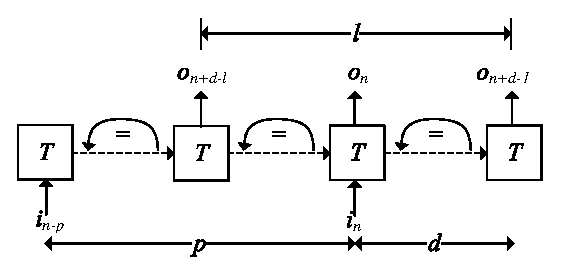
\includegraphics[width=0.45\textwidth]{doubleloop}
%\end{center}
%\caption{The loop-like non-complementary condition}
%  \label{fig_double_loop_again}
%\end{figure}
%
%\begin{figure}[b]
%\begin{center}
%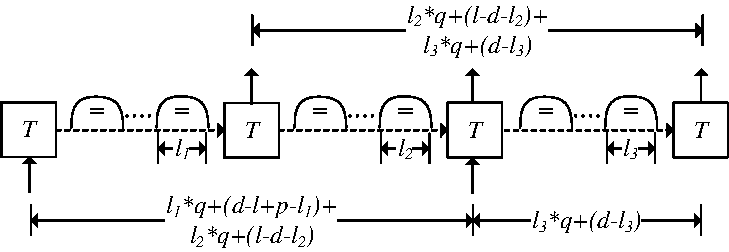
\includegraphics[width=0.45\textwidth]{doubleloop_unfold}
%\end{center}
%\caption{The loop-like non-complementary condition unfolded for $q$ times}
%  \label{fig_double_loop_unfold}
%\end{figure}
%
%We first need to define how to unfold the three loops in Figure \ref{fig_double_loop_again}.
%Assume the length of loops in $Prefix_{p,d,l}$, $Left_{p,d,l}$ and $Right_{p,d,l}$ are $l_1$, $l_2$ and $l_3$ respectively.
%Further assume they are unfolded for $q$ times.
%Then,
%the SAT instance generated from this unfolding is shown in Figure \ref{fig_double_loop_unfold}.
%It is obvious that,
%the unfolded SAT instance corresponds to $F_{LN}(p",d",l",R)$,
%where:
%
%\begin{equation}
%\begin{array}{ccc}
%p"&=&l_1*q+(d-l+p-l_1)+l_2*q+(l-d-l_2) \\
%d"&=&l_3*q+(d-l_3) \\
%l"&=&l_2*q+(l-d-l_2)+l_3*q+(d-l_3)
%\end{array}
%\end{equation}
%
%Obviously,
%for every particular $<p,d,l>$ and $<p',d',l'>$,
%there always exists a $q$,
%such that $Prefix_{p",d",l"}$, $Left_{p",d",l"}$ and $Right_{p",d",l"}$ resulted from this unfolding
%are \emph{not shorter} than $Prefix_{p',d',l'}$,$Left_{p',d',l'}$ and $Right_{p',d',l'}$ respectively.
%
%
%
%% \subsection{Proving correctness}\label{subsec_correctness}
%
%We then need to prove some lemmas about this unfolded SAT instance.
%\begin{figure}[b]
%\centering
%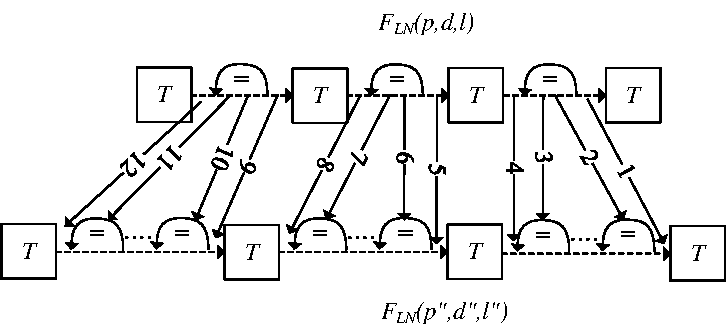
\includegraphics[width=0.45\textwidth]{doubleloop_unfold_cmp}
%\caption{Correspondance between $F_{LN}(p,d,l,R)$ and $F_{LN}(p",d",l",R)$}
%\label{doubleloop_unfold_cmp}
%\end{figure}
%
%\begin{lemma}[]\label{lemma_unfold_longer}
%For $F_{LN}(p",d",l",R)$ in Figure \ref{fig_double_loop_unfold},
%we have $F_{LN}(p,d,l,R)\to F_{LN}(p",d",l",R)$
%\end{lemma}
%\begin{proof}
%The formula $F_{LN}(p",d",l",R)$ is:
%
%\begin{equation}\label{equ_correspondance}
%\begin{split}
%&F_{LN}(p",d",l",R)\stackrel{def}{=}\\
%&\left\{
%\begin{array}{cc}
%&\bigwedge_{m=n-p"}^{n+d"-1}
%\{
%(s_{m+1},o_m)\equiv T(s_m,i_m,c_m)
%\}
%\\
%\wedge&\bigwedge_{m=n-p"}^{n+d"-1}
%\{
%(s'_{m+1},o'_m)\equiv T(s'_m,i'_m,c'_m)
%\}
%\\
%\wedge&\bigwedge_{m=n+d"-l"}^{n+d"-1}o_m\equiv o'_m \\
%\wedge& i_n\ne i'_n \\
%\wedge&\bigwedge_{x=n-p"}^{n+d"-1}c_x\equiv c \\
%\wedge&\bigwedge_{x=n-p"}^{n+d"-1}c_x'\equiv c \\
%\wedge& R(c) \\
%\wedge& \bigvee_{x=n-p"}^{n+d"-l"-1}\bigvee_{y=x+1}^{n+d"-l"} \{s_x\equiv s_y\wedge s'_x\equiv s'_y\} \\
%\wedge& \bigvee_{x=n+d"-l"+1}^{n-1}\bigvee_{y=x+1}^{n} \{s_x\equiv s_y\wedge s'_x\equiv s'_y\} \\
%\wedge& \bigvee_{x=n+1}^{n+d"-1}\bigvee_{y=x+1}^{n+d"} \{s_x\equiv s_y\wedge s'_x\equiv s'_y\}
%\end{array}
%\right\}
%\end{split}
%\end{equation}
%
%Assume that $F_{LN}(p,d,l,R)$ is satisfied,
%and its satisfying assignment is $A$.
%We need to prove that $F_{LN}(p",d",l",R)$ is also satisfied with $A$.
%
%The directed arcs numbered from 1 to 12 in Figure \ref{doubleloop_unfold_cmp},
%show the correspondence between $F_{LN}(p,d,l,R)$ and the $F_{LN}(p",d",l",R)$.
%
%The arcs 2 and 3 mean that we can apply the satisfying assignment of the loop in $Right_{p,d,l}$
%to the unfolded loops in $Right_{p",d",l"}$.
%The arcs 1 and 4 mean that we can apply the the satisfying assignments of the two paths not in the loop,
%to $Right_{p",d",l"}$.
%With the arcs from 1 to 4,
%we can make the path $Right_{p",d",l"}$ satisfiable.
%
%Similarly,
%we can also make $Prefix_{p",d",l"}$ and $Left_{p",d",l"}$ satisfiable.
%Thus the 2nd line of Equation (\ref{equ_correspondance}) is satisfied with the assignment $A$.
%Similarly,
%the 3rd to 8th lines of Equation (\ref{equ_correspondance}) are also satisfied with the assignment $A$.
%
%At the same time,
%there are $q$ loops in $Prefix_{p",d",l"}$, $Left_{p",d",l"}$ and $Right_{p",d",l"}$,
%which will make the last three lines in Equation (\ref{equ_correspondance}) satisfied.
%
%Thus,the satisfying assignment $A$ of $F_{LN}(p,d,l,R)$ can also make $F_{LN}(p",d",l",R)$ satisfied.
%This concludes the proof.
%\end{proof}
%
%\begin{lemma}[]\label{lemma_pc_long}
%For two tuples $<p,d,l>$ and $<p',d',l'>$,
%if $Prefix_{p',d',l'}$,$Left_{p',d',l'}$ and $Right_{p',d',l'}$ are \emph{not shorter} than $Prefix_{p,d,l}$,$Left_{p,d,l}$ and $Right_{p,d,l}$ respectively,
%then $E\vDash PC(p,d,l,R)\to E\vDash PC(p',d',l',R)$.
%\end{lemma}
%\begin{proof}
%It is obvious that $F_{PC}(p,d,l,R)$ is a sub-formula of $F_{PC}(p',d',l',R)$,
%which means the unsatisfiability of the former implies the unsatisfiability of the latter.
%Thus,
%$E\vDash PC(p,d,l,R)\to E\vDash PC(p',d',l',R)$ holds.
%\end{proof}
%
%The following two theorems will prove that $E\vDash LN(R)\leftrightarrow \neg \{E\vDash PC(R)\}$.
%
%\begin{theorem}\label{thm_pc_nln}
%$E\vDash LN(R)\to \neg \{E\vDash PC(R)\}$
%\end{theorem}
%\begin{proof}
%We can prove it by contradiction.
%Assume that $E\vDash LN(R)$ and $E\vDash PC(R)$ both hold.
%This means there exist $<p,d,l>$ and $<p',d',l'>$,
%such that $E\vDash PC(p,d,l,R)$ and $E\vDash LN(p',d',l',R)$.
%
%On one hand,
%$E\vDash LN(p',d',l',R)$ means there are loops in $Prefix_{p',d',l'}$,$Left_{p',d',l'}$ and $Right_{p',d',l'}$.
%By unfolding these loops,
%we get another tuple $<p",d",l">$,
%such that :
%\begin{enumerate}
%\item $Prefix_{p",d",l"}$,$Left_{p",d",l"}$ and $Right_{p",d",l"}$ are longer than $Prefix_{p,d,l}$,$Left_{p,d,l}$ and $Right_{p,d,l}$ respectively
%\item According to Lemma \ref{lemma_unfold_longer},
%$F_{LN}(p",d",l",R)$ is satisfiable.
%\end{enumerate}
%
%$F_{PC}(p",d",l",R)$ is a sub-formula of $F_{LN}(p",d",l",R)$,
%so $F_{PC}(p",d",l",R)$ is also satisfiable,
%which means that $E\vDash PC(p",d",l",R)$ does not hold.
%
%On the other hand,
%according to Lemma \ref{lemma_pc_long},
%$E\vDash PC(p",d",l",R)$ holds.
%This contradiction concludes the proof.
%\end{proof}
%
%\begin{theorem}\label{thm_nln_pc}
%$E\vDash LN(R)\gets \neg \{E\vDash PC(R)\}$
%\end{theorem}
%\begin{proof}
%We can also prove it by contradiction.
%Assume that neither $E\vDash LN(R)$ nor $E\vDash PC(R)$ holds.
%Then for every $<p,d,l>$ and $<p',d',l'>$,
%$F_{PC}(p,d,l,R)$ is satisfiable,
%while $F_{LN}(p',d',l',R)$ is unsatisfiable.
%
%Thus,
%assume $uirrd(M^2)$ is the uninitialized state variables recurrence diameter of $E$'s product machine.
%Let's define $<p,d,l>$ as:
%\begin{equation}
%\begin{array}{c}
%p=uirrd(M^2)*2+2 \\
%d=uirrd(M^2)+1 \\
%l=uirrd(M^2)*2+2
%\end{array}
%\end{equation}
%
%With this definition,
%it is obvious that $Prefix_{p,d,l}$,$Left_{p,d,l}$ and $Right_{p,d,l}$ are all longer than $uirrd(M^2)$.
%This means there are loops in all these three paths,
%which will make $F_{LN}(p,d,l,R)$ satisfiable.
%This contradicts with the fact that $F_{LN}(p',d',l',R)$ is unsatisfiable for every $<p',d',l'>$.
%This contradiction concludes the proof.
%\end{proof}
%
%With Theorem \ref{thm_pc_nln} and \ref{thm_nln_pc},
%Theorem \ref{thm_pcln_exclusive} is proved.

% use section* for acknowledgement
%\section*{Acknowledgment}
% The authors would like to thank the editors and anonymous reviewers for their hard work.

%This work was funded by projects 60603088 and 61070132 supported by National Natural Science Foundation of China.


%The authors would like to thank the anonymous reviewer's time and effort.

%This work is fund by Chinese National Science Foundation No.60603088.


% Can use something like this to put references on a page
% by themselves when using endfloat and the captionsoff option.
\ifCLASSOPTIONcaptionsoff
  \newpage
\fi



% trigger a \newpage just before the given reference
% number - used to balance the columns on the last page
% adjust value as needed - may need to be readjusted if
% the document is modified later
%\IEEEtriggeratref{8}
% The "triggered" command can be changed if desired:
%\IEEEtriggercmd{\enlargethispage{-5in}}

% references section

% can use a bibliography generated by BibTeX as a .bbl file
% BibTeX documentation can be easily obtained at:
% http://www.ctan.org/tex-archive/biblio/bibtex/contrib/doc/
% The IEEEtran BibTeX style support page is at:
% http://www.michaelshell.org/tex/ieeetran/bibtex/
% \bibliographystyle{IEEEtran}
% argument is your BibTeX string definitions and bibliography database(s)
% \bibliography{IEEEabrv,sigproc}
%
% <OR> manually copy in the resultant .bbl file
% set second argument of \begin to the number of references
% (used to reserve space for the reference number labels box)
 \begin{thebibliography}{19}
\bibitem{ShengYuShen:iccad09}
S.~Shen, J.~Zhang, Y.~Qin, and S.~Li, ``Synthesizing complementary circuits
  automatically,'' in \emph{ICCAD09}.\hskip 1em plus 0.5em minus 0.4em\relax
  IEEE, Nov. 2009, pp. 381--388.

% \bibitem{ShengYuShen:iccad11}
% S.~Shen, J.~Zhang, Y.~Qin, and S.~Li, ``Inferring Assertion for Complementary
%  Synthesis,''\emph{accepted by ICCAD11.
%   \url{http://www.ssypub.org/pub/iccad11_ssy.pdf}}.
\bibitem{ShengYuShen:iccad11}
S.~Shen, Y.~Qin, J.~Zhang, and S.~Li, ``Inferring Assertion for Complementary
 Synthesis,''in \emph{ICCAD11}.\hskip 1em plus 0.5em minus 0.4em\relax
  ACM, Nov. 2011, pp. 404--411.

\bibitem{PCIESPEC}
"PCI Express Base Specification Revision 1.0". [Online]. Available:
  \url{http://www.pcisig.com}

\bibitem{IEEE80232002}
"IEEE Standard for Information technology Telecommunications and
  information exchange between systems Local and metropolitan area networks
  Specific requirements Part 3: Carrier Sense Multiple Access with Collision
  Detection (CSMA/CD) Access Method and Physical Layer Specifications
  Amendment: Media Access Control (MAC) Parameters, Physical Layers, and
  Management Parameters for 10 Gb/s Operation", IEEE Std. 802.3, 2002.

\bibitem{funcdep}
C.-C. Lee, J.-H.~R. Jiang, C.-Y. Huang, and A.~Mishchenko, ``Scalable
  exploration of functional dependency by interpolation and incremental SAT
  solving,'' in \emph{ICCAD07}.\hskip 1em plus 0.5em minus 0.4em\relax IEEE,
  Nov. 2007, pp. 227--233.

%\bibitem{CHAFF}
%M. W. Moskewicz, C. F. Madigan, Y. Zhao, L. Zhang, and S. Malik.
%\newblock Chaff: Engineering an Efficient SAT Solver.
%\newblock In {\em DAC01}, pages 530--535. IEEE, June
%  2001.
%
%\bibitem{grasp}
%J. P. M. Silva and K. A. Sakallah.
%\newblock GRASP - a new search algorithm for satisfiability.
%\newblock In {\em ICCAD96}, pages 220--227. IEEE, November
%  1996.
%
%\bibitem{BERKMIN}
%E. Goldberg and Y. Novikov.
%\newblock BerkMin: a fast and robust SAT-solver.
%\newblock In {\em DATE02}, pages 142--149. IEEE, March
%  2002.

\bibitem{EXTSAT}
N.~E\'en and N.~S\"orensson.
\newblock An extensible sat-solver.
\newblock In {\em SAT03}, pages 502--518. Springer, May
  2003.

\bibitem{Cofact}
M.~K. Ganai, A.~Gupta, and P.~Ashar, ``Efficient SAT-based unbounded symbolic
  model checking using circuit cofactoring,'' in \emph{ICCAD04}.\hskip 1em plus
  0.5em minus 0.4em\relax IEEE, Nov. 2004, pp. 510--517.

% \bibitem{Craig}
% W.~Craig, ``Linear reasoning: A new form of the Herbrand-Gentzen theorem,''
%   \emph{J. Symbolic Logic}, vol.~22, no.~3, pp. 250--268, 1957.

\bibitem{interp_McMillan}
K.~L. McMillan, ``Interpolation and SAT-based model checking,'' in
  \emph{CAV03}.\hskip 1em plus 0.5em minus 0.4em\relax Springer, July 2003, pp.
  1--13.

%\bibitem{MEALY}
%G.~H. Mealy, ``A method for synthesizing sequential circuits,'' \emph{Bell
%  Systems Technical Journal}, vol.~34, no.~5, pp. 1045--1079, 1955.

%\bibitem{RecDiam}
%D.~Kroening and O.~Strichman, ``Efficient computation of recurrence
%  diameters,'' in \emph{VMCAI03}.\hskip 1em plus 0.5em minus 0.4em\relax
%  Springer, January 2003, pp. 298--309.

\bibitem{ShengYuShen:tcad}
S.~Shen, Y.~Qin, K.~Wang, L.~Xiao, J.~Zhang, and S.~Li, ``Synthesizing
  complementary circuits automatically,'' \emph{IEEE trans. on CAD of
  Integrated Circuits and Systems}, vol.~29, no.~8, pp. 1191--1202, Aug.
  2010.

\bibitem{ShengYuShen:tcad11}
S.~Shen, Y.~Qin, L.~Xiao, K.~Wang, J.~Zhang, and S.~Li, ``A halting algorithm
  to determine the existence of the decoder,'' \emph{IEEE trans. on CAD of
  Integrated Circuits and Systems}, vol.~30, no.~10, pp. 1556--1563, Oct.
  2011.

\bibitem{Roland:iccad11}
S. Liu, Y. Chou, C. Lin, and J. Jiang, ``Towards completely automatic decoder synthesis,''
in \emph{ICCAD11}.\hskip 1em plus 0.5em minus 0.4em\relax
  ACM, Nov. 2011, pp. 389--395.


%\bibitem{ShengYuShen:fmcad10}
%S.~Shen, Y.~Qin, J.~Zhang, and S.~Li, ``A halting algorithm to determine the
%  existence of decoder,'' in \emph{FMCAD10}.\hskip 1em plus 0.5em minus
%  0.4em\relax IEEE,  Oct. 2010, pp. 91--100.

%\bibitem{dim_syn}
%S.~Gulwani, ``Dimensions in program synthesis,'' in \emph{PPDP10}.\hskip 1em
%  plus 0.5em minus 0.4em\relax ACM, July 2010, pp. 13--24.
%
%\bibitem{prog_inv}
%E.~W. Dijkstra, ``Program inversion,'' in \emph{Program Construction 1978},
%  1978, pp. 54--57.
%
%\bibitem{mtd_autoProginv}
%R.~Gl\"uck and M.~Kawabe, ``A method for automatic program inversion based on
%  lr(0) parsing,'' \emph{Fundam. Inf.}, vol.~66, no.~4, pp. 367--395, Nov.
%  2005.
%
%\bibitem{prog_inv_rev}
%S.~Srivastava, S.~Gulwani, S.~Chaudhuri, and J.~Foster, ``Program inversion
%  revisited,'' \emph{MSR-TR-2010-34, Microsoft Research},
%  2010.

%\bibitem{YexinZheng_aspdac09}
%Y.~Zheng, and C.~Huang, ``A novel Toffoli network synthesis algorithm for reversible logic,''
%in \emph{ASPDAC09}. IEEE, Jan. 2009, pp. 739--744.

%\bibitem{RobertWille_dac10}
%R.~Wille, M.~Soeken, and R.~Drechsler, ``Reducing the number of lines in reversible circuits,''
%in \emph{DAC10}. IEEE, Jun. 2010, pp. 647--652.
%
%\bibitem{VivekVShende_tcad03}
%V.~Shende, A.~Prasad, I.~Markov, and J.~Hayes, ``Synthesis of reversible logic circuits,''
%\emph{IEEE transaction on CAD of
%  Integrated Circuits and Systems}, vol.~22, no.~6, pp. 710--722, Jun.
%  2003.
%
%\bibitem{WilliamHung_dac04}
%W.~Hung, X.~Song, G.~Yang, J.~Yang, and M.~Perkowski, ``Quantum logic synthesis by symbolic reachability analysis, ``
%in \emph{DAC04}. IEEE, Jun. 2004, pp. 838--841.
%
%\bibitem{Kerntopf_dac04}
%P.~Kerntopf, ``A new heuristic algorithm for reversible logic
%synthesis, ``
%in \emph{DAC04}. IEEE, Jun. 2004, pp. 834--837.
%
%\bibitem{Maslov_tcad05}
%D.~Maslov, G.~Dueck, and D.~Miller, ``Toffoli network
%synthesis with templates, ``
%\emph{IEEE transaction on CAD of
%  Integrated Circuits and Systems}, vol.~24, no.~6, pp. 807--817, Jun.
%  2005.

%\bibitem{Gupta_tcad06}
%P.~Gupta, A.~Agrawal, and N.~Jha, ``An algorithm for
%synthesis of reversible logic circuits, ``
%\emph{IEEE transaction on CAD of
%  Integrated Circuits and Systems}, vol.~25, no.~11, pp. 2317--2330, Nov.
%  2006.
%
%\bibitem{Maslov_tcad11}
%D.~Maslov, and M.~Saeedi, ``Reversible Circuit Optimization Via Leaving the Boolean Domain, ``
%\emph{IEEE transaction on CAD of
%  Integrated Circuits and Systems}, vol.~30, no.~6, pp. 806--816, Jun.
%  2011.

\bibitem{converter_date08}
K.~Avnit, V.~D'Silva, A.~Sowmya, S.~Ramesh, and S.~Parameswaran, ``A formal
  approach to the protocol converter problem,'' in \emph{DATE08}.\hskip 1em
  plus 0.5em minus 0.4em\relax IEEE, Mar. 2008, pp. 294--299.

%\bibitem{converter_date09}
%K.~Avnit and A.~Sowmya, ``A formal approach to design space exploration of
%  protocol converters,'' in \emph{DATE09}.\hskip 1em plus 0.5em minus
%  0.4em\relax IEEE, Mar. 2009, pp. 129--134.
 \end{thebibliography}

% that's all folks
\end{document}


